%/**
% * @file tese.tex
% * @brief This file have the configuration parameters of Dr. Degree thesis.
% * @ingroup Documentation
% * @author $Author: rodcosta $
% * @date $Date: 2009/07/12 18:54:10 $
%**
\documentclass[12pt,a4paper,oneside,final]{book}
%%% para vers\~{o}es parciais do dumento final utilizar:
%\documentclass[12pt,a4paper,draft]{book}
%\documentclass[12pt,a4paper,twoside,fleqn,draft]{book}
%%%%%%%%%%%%%%%%%%%%%%%%%%%%%%%%%%%%%%%%%%%%%%%%%%%%%%%%%%%%%%%%
%%% PREAMBULO DO DOCUMENTO COME\c{C}A AQUI
%\usepackage{natbib}
%\bibliographystyle{elsart-harv}
%inclui coisas da abnt
%\bibliographystyle{abntcite}
%\usepackage{hvfoat}
\usepackage{datetimepor}
\usepackage{monografia}
\usepackage{multicol}
\usepackage{rotating}
\usepackage{monografia_defs}
\usepackage[none]{hyphenat}
\usepackage[latin1]{inputenc}
\usepackage{assinatura}
\usepackage{color}
\usepackage{multirow}
% \bibstyle{abnt-alf}
\usepackage{sidecap}
\usepackage{ifthen}
\usepackage{psfrag}
\usepackage{supertabular}
\usepackage[subfigure]{tocloft}

% Permite utilizar configuracoes da linguagem portugesa do Brasil e Inglesa
\usepackage[english,brazil]{babel}
% Permite especificar codificacao das entradas (caracteres acentuados - � - sem usar \'a)
%\usepackage[latin1]{inputenc}
% Permite utiliza��o de referencias cruzadas
\usepackage[brazil]{varioref}
\usepackage[T1]{fontenc}
%
\usepackage{listings}             % Include the listings-package




\newcommand{\titulo}{iQuizzer: Estudo de caso para integra��o entre aplica��es Web e dispositivos m�veis}
\newcommand{\autor}{Tiago Augusto da Silva Bencardino}
\newcommand{\orientador}{Prof. Dr. Jos� Marques Soares}
\newcommand{\coorientador}{Prof. }
\newcommand{\membroa}{Prof. p1}
\newcommand{\membrob}{Prof. p2}
\newcommand{\membroc}{Prof. p3}
\renewcommand{\eqref}[1]{equa\c{c}\~{a}o~\ref{#1}}
\newcommand{\eqrefp}[1]{equa\c{c}\~{o}es~\ref{#1}}
\newcommand{\ok}{$\blacksquare$}
\newcommand{\nok}{$\square$}

\newcommand{\secao}{\section}
\newcommand{\capitulo}{\chapter}
\newcommand{\subsecao}{\subsection}

\newcommand{\secref}[1]{se\c{c}\~{a}o~\ref{#1}}
\newcommand{\secrefp}[1]{se\c{c}\~{o}es~\ref{#1}}
\newcommand{\tabref}[1]{Tabela~\ref{#1}}
\newcommand{\tabrefp}[1]{Tabelas~\ref{#1}}
\newcommand{\figref}[1]{Figura~\ref{#1}}
\newcommand{\figrefp}[1]{Figuras~\ref{#1}}
\newcommand{\quadro}[1]{Quadro~\ref{#1}}
\usepackage[breaklinks,final,pdftitle={\titulo},pdfauthor = {\autor}]{hyperref}

%\usepackage{hyperref}
\usepackage[sort]{cite}
\usepackage[alf,abnt-and-type=e,abnt-full-initials=no,abnt-last-names=abnt,abnt-etal-list=2,abnt-etal-text = emph]{abntcite}
\newcommand{\citet}[1]{\citeonline{#1}}

%\newcommand{\eqref}[1]{(\ref{#1})}
\newcolumntype{Y}{>{\centering\arraybackslash}X}
%\newcommand{\secref}[1]{se\c{c}\~{a}o~\ref{#1}}
%\newcommand{\secrefp}[1]{se\c{c}\~{o}es~\ref{#1}}
%\newcommand{\tabref}[1]{Tabela~\ref{#1}}
%\newcommand{\tabrefp}[1]{Tabelas~\ref{#1}}
%\newcommand{\figref}[1]{Figura~\ref{#1}}
%\newcommand{\figrefp}[1]{Figuras~\ref{#1}}
%
%\usepackage[dvips]{graphicx}
%\usepackage[portuges]{babel}
\usepackage[printonlyused]{acronym}
\usepackage{hvfloat}

\usepackage{tabularx}
\usepackage{here}
\usepackage{listings}
% Definindo novos tipos de lista
\usepackage{tocloft}
\usepackage{etoolbox}
%\newcommand{\listexamplename}{\textbf{\Huge{Lista de Quadros}}}
%\newlistof{example}{exp}{\listexamplename}
%\newcommand{\example}[1]{%
%    \refstepcounter{example}
%    \par\noident\textbf{Quadro \theexample.#1}
%    \addcontentsline{exp}{example}
%    {\protect\numberline{\theexample}#1}\par
%}
%
    \usepackage{longtable}
\usepackage{supertabular}

\hyphenation{defei-tuoso Fe-de-ral Uni-ver-si-da-de Dis-cos atri-bu-tos re-sul-ta-dos ar-ma-ze-na-men-to}
\hyphenation{tem-pe-ra-tu-ra sis-te-ma lei-tu-ra }

%\usepackage[num]{abntcite} %saint
\begin{document}
%padronizacao
\DeclareGraphicsExtensions{.jpg,.pdf,.mps,.png}

%\usepackage[final]{pdfpages}
%\usepackage{Fancyhdr}
%\bibliographystyle{IEEEtranPor}
% \includeonly{capa,agradecimentos}
% \includeonly{capa_externa,capa}
%%% PREAMBULO DO DOCUMENTO ACABA AQUI
%%%%%%%%%%%%%%%%%%%%%%%%%%%%%%%%%%%%%%%%%%%%%%%%%%%%%%%%%%%%%%%%

%%%%%%%%%%%%%%%%%%%%%%%%%%%%%%%%%%%%%%%%%%%%%%%%%%%%%%%%%%%%%%%%
%%% CAPA

\pagenumbering{Roman}
\thispagestyle{empty}%

\begin{center}
    
\includegraphics[width=2.5cm]{figs/ufc.jpg} \\%
    \textsc{
    Universidade Federal do Cear� \\%
    Departamento de Engenharia de Teleinform�tica \\%
    Curso de Gradua��o em Engenharia de Teleinform�tica\\
    }
    \vspace{2.5 cm}%
    {       \textbf{\autor}
    }\\%

    \null\vfill%%
    \vspace{.2cm}%
    {\Large         \textbf{\titulo}\\}


    \null\vfill%%
    \vspace{1 cm}%
    {\normalsize    \textsc{Fortaleza -- Cear� \\%
                            Dezembro~2011 }}
\end{center}

% ----------------------------------------------------------------------- %
% Onde serão inseridas informações que irão aparecer na capa e na
% folha de rosto
%
% Arquivo: capa.tex
% ----------------------------------------------------------------------- %
%\capa
%%capa feita manualmente
%%-------------------------
\begin{titlepage}
\begin{center}

\includegraphics[scale=0.33]{fig/logo_UFC.eps}\\
\vfill
{\MakeUppercase{\instituicao}}\par
{\MakeUppercase{\departamento}}\par
{\MakeUppercase{\curso}}\\
\vfill
\begin{center}
\Large\MakeUppercase{\titulo}\par
\end{center}
\vfill\vfill
\begin{center}
{\MakeUppercase{\autor}}
\end{center}
\vfill\vfill\vfill

\setlength{\parskip}{.3cm}
{\normalfont{\Local}} \par
{\normalfont{\Data}}
\end{center}
\end{titlepage}
%%-------------------------
%Folha de rosto feita manualmente
%----------------------------------------
\thispagestyle{empty}
\vspace{1.1cm}
  \begin{center}
    \MakeUppercase{\autor}
  \end{center}
\vfill\vfill\vfill
   \begin{center}
     \Large\MakeUppercase{\titulo}\par
   \end{center}
   \vspace{.8cm}
   \hspace{.45\textwidth}
     \begin{minipage}{.5\textwidth}
         {\comentario}\par
     \end{minipage}
\vspace{.8cm}
\begin{center}
   Orientador: {\orientador}
   \vspace{0.7cm}
   \end{center}
\vfill
\begin{center}
  \setlength{\parskip}{.3cm}
     \setlength{\parskip}{0cm}
     {\MakeUppercase{\instituicao}}\par
	{\MakeUppercase{\departamento}}\par
	{\MakeUppercase{\curso}}\\
     \setlength{\parskip}{.3cm}\par
\end{center}
\vfill\vfill
\begin{center}
\setlength{\parskip}{.3cm}
{\normalfont{\Local}} \par
{\normalfont{\Data}}
\end{center}

%---------------------------------------
\thispagestyle{empty}%

\begin{center}
    %
\includegraphics[width=2.5cm]{figs/UFC.eps} \\%
    \textsc{ \autor } \\
     \vspace{.5 cm} \textbf{ \titulo }     \\
\end{center}
    \vspace{.2 cm}
    Esta Monografia foi julgada adequada para a obten��o do diploma de Engenheira do Curso de Gradua��o em Engenharia de Teleinform�tica da Universidade Federal do Cear�.
    \assinatura{\autor}
    \vspace{0.2 cm}
     Banca Examinadora:
     \assinatura{\orientador \\ Orientador}
     \assinatura{\membroa\\}
     \assinatura{\membrob \\}
    \assinatura{\membroc\\}
%     \assinatura{\membrod}
     \vspace{0.2 cm}%\null\vfill%%

\begin{center}
    {\normalsize    Fortaleza, \today}
\end{center}

\frontmatter \pagestyle{roman}
%%%%%%%%%%%%%%%%%%%%%%%%%%%%%%%%%%%%%%%%%%%%%%%%%%%%%%%%%%%%%%%%
%%% RESUMO

% ----------------------------------------------------------------------- %
% Pequeno texto que em poucas palavras consegue expressar o trabalho.
% O resumo deve ser concebido de forma tal que, uma pessoa ao ler o resumo
% possa entender sobre qual assunto este trabalho trata.
%
% Arquivo: resumo.tex
% ----------------------------------------------------------------------- %
\pdfbookmark[1]{Resumo}{CHP:RESUM0}
\chapter*{Resumo}
\label{CHP:RESUM0}
\thispagestyle{empty}
\singlespacing
	\lipsum[3-4]
\onehalfspacing
\pdfbookmark[1]{Abstract}{CHP:ABSTRACT}
\chapter*{Abstract}
\label{CHP:ABSTRACT}%%
\thispagestyle{empty}


\PARstartOne{A} great number of web applications has, for mobile platforms \emph{iOS} and \emph{Android}, some version for mobile systems, which same information is shared on cloud. Some popular social networks like \emph{Twitter} and \emph{Foursquare} has communication interfaces REST as a service to other applications. This paper aims to make a comparative study between iOS and Android applications that use a RESTful web application. To conduct the study, it created a small social network to create quizzes using \emph{Ruby on Rails} and a SaaS service like \emph{Heroku}.


%\PARstartOne{H}{ard} disks are very important elements in any modern computer system and it is advisable to monitor the health of these devices because they are used for applications from personal computers to risk activities. This work aims to build a framework in Linux system using the standard commands \ac{ATA} and \ac{SCSI} to support the development of algorithms for test drives. To demonstrate the use of the framework, algorithms are implemented some test that is compared with diagnostic tools on the market. Finally, these algorithms are embedded in a bootable version of Linux, which allows you to perform during any computers that support booting from a live CD or USB stick, regardless of operating system installed. The test results show the algorithm is very satisfactory, demonstrating the effectiveness of the framework.

%For the development of the work all commands have been developed in ANSI C + + language. Several commands \ac{ATA} and \ac{SCSI} were implemented to support reading, self-testing and other features. Also, the algorithm are implemented from them.
%\newline
%\newline
\noindent \textbf{Keywords: iOS, Android, Mobile, Ruby on Rails, REST, RESTFul}.

%Hard disks are  elements in any modern computer system and it is  to monitor the health of these devices, because they are used for applications from personal computer to risk activities. This work aims to build a framework in Linux system using the standard commands ATA and SCSI to support the development of algoritms for test devices. 
%%%%%%%%%%%%%%%%%%%%%%%%%%%%%%%%%%%%%%%%%%%%%%%%%%%%%%%%%%%%%%%%
%%% DEDICATRIA
% ----------------------------------------------------------------------- %
% Pequena dedicatória ou uma epígrafe (uma citação pertinente ao seu 
% trabalho ou que represente o seu modo de pensar.) 
% 
%
% Arquivo: dedicatoria.tex
% ----------------------------------------------------------------------- %
\thispagestyle{empty}
\vspace*{\fill}

{ \raggedleft


\textit{Dedico este trabalho a ...}

~
}

%%%%%%%%%%%%%%%%%%%%%%%%%%%%%%%%%%%%%%%%%%%%%%%%%%%%%%%%%%%%%%%%
%%% AGRADECIMENTOS
%\chapter{Agradecimentos}
\label{CHP:ACKNOWLEDGMENT}%%
\thispagestyle{empty}
% \PARstartOne{A}{grade\c{c}o}
%Agrade\c{c}o primeiramente ao Pai Celestial por todas as ben\c{c}\~{a}os derramadas sobre mim
%durante toda minha vida.
%
%\`{A} minha esposa que est\'{a} sempre me apoiando desde a escrita da minha Monografia na gradua\c{c}\~{a}o.
%
%Ao Professor Dr. Paulo C\'{e}sar Cortez, meu Orientador Cient\'{\i}fico, pela amizade e a oportunidade de receber um pouco de sua sabedoria, pela disponibilidade
%apresentada e pelas condi\c{c}\~{o}es que me proporcionou para a realiza\c{c}\~{a}o
%deste trabalho.
%
%Ao Rodrigo Costa, pela paci\^{e}ncia e esfor\c{c}o compartilhado auxiliando na orienta\c{c}\~{a}o desse trabalho, e aos demais integrantes do grupo GIHM (Grupo de Inova\c{c}\~{a}o ).
%
%Aos amigos, Auzuir Ripardo, Pedro Pedrosa , Tarique Cavalcante, dentre
%outros integrantes do sub-grupo de pesquisa em Engenharia Biom\'{e}dica do Laborat\'{o}rio de Engenharia de Sistemas de Computa\c{c}\~{a}o, pela amizade e esfor\c{c}o compartilhado durante o curso de mestrado.
%
%Aos engenheiros de desenvolvimento do SIDI (Samsung Instituto de Desenvolvimento para a Inform\'{a}tica), Giovanni, Miguel e Nelson pelo embarque dos algoritmos na plataforma de testes.
%
%Por fim, mas n\~{a}o menos importante, \`{a} Coordena\c{c}\~{a}o de Aperfei\c{c}oamento de Pessoal de N\'{\i}vel Superior (CAPES) e Funda\c{c}\~{a}o Cearense de Apoio ao Desenvolvimento Cient\'{\i}fico e Tecnol\'{o}gico (FUNCAP) pelo suporte financeiro atrav\'{e}s do concedimento da bolsa de Mestrado.


%\textbf{DEDICAT\'{O}RIA}
\thispagestyle{empty}%
\newpage
\null\vfill
\begin{flushright}
%\emph{"Fazer do of\'{\i}cio uma divers\~{a}o levada a s\'{e}rio."}\\Chico Science
\emph{$\ldots$ Cada sonho que voc� deixa pra tr�s, � um peda�o do seu futuro que deixa de existir.}\\
Steve Jobs

%\emph{ "$\ldots$\\All your life, You were only waiting for the moment to arise.\\
%%...
%%All your life, You were only waiting for the moment to be free.
%Black bird fly, black bird fly\\
%Into the light of the dark black night\\$\ldots$" }
%
%\emph{Black Bird - The Beatles}
\end{flushright}
   \vspace{3.0cm}

%% ----------------------------------------------------------------------- %
% Pequena dedicatória ou uma epígrafe (uma citação pertinente ao seu 
% trabalho ou que represente o seu modo de pensar.) 
% 
%
% Arquivo: dedicatoria.tex
% ----------------------------------------------------------------------- %
\thispagestyle{empty}
\vspace*{\fill}

{ \raggedleft


\textit{Dedico este trabalho a ...}

~
}

%%%%%%%%%%%%%%%%%%%%%%%%%%%%%%%%%%%%%%%%%%%%%%%%%%%%%%%%%%%%%%%%
%%% ABREVIA\c{C}\~{O}ES
\begin{singlespace}
    %%%%%%%%%%%%%%%%%%%%%%%%%%%%%%%%%%%%%%%%%%%%%%%%%%%%%%%%%%%%%%%%
    %%% \'{I}NDICE
    %\addtocontents{toc}{\noindent\protect\rule{\textwidth}{.2pt}\par}
    \pdfbookmark[1]{Sum�rio}{sumario_label} %\label{sumario_label}
    \tableofcontents%
    %%%%%%%%%%%%%%%%%%%%%%%%%%%%%%%%%%%%%%%%%%%%%%%%%%%%%%%%%%%%%%%%
    %%% LISTA DE FIGURAS
    \newpage
    %\pdfbookmark[1]{Lista de Figuras}
    \listoffigures%
    \addcontentsline{toc}{chapter}{Lista de Figuras}%
    %%%%%%%%%%%%%%%%%%%%%%%%%%%%%%%%%%%%%%%%%%%%%%%%%%%%%%%%%%%%%%%%
    %%% LISTA DE TABELAS
    \newpage
    \listoftables%
    \addcontentsline{toc}{chapter}{Lista de Tabelas}%
    %%%%%%%%%%%%%%%%%%%%%%%%%%%%%%%%%%%%%%%%%%%%%%%%%%%%%%%%%%%%%%%%
    %%% LISTA DE QUADROS
  %  \newpage
%    \addcontentsline{toc}{chapter}{Lista de Quadros}%
%    \chapter*{Lista de Quadros}%%
%    
Quadro 1

Quadro 2

Quadro 3

    %%%%%%%%%%%%%%%%%%%%%%%%%%%%%%%%%%%%%%%%%%%%%%%%%%%%%%%%%%%%%%%%
    %%% LISTA DE ALGORITMOS
    %    \listofalgorithms%
    %    \addcontentsline{toc}{chapter}{Lista de Algoritmos}%
     %\addtocontents{toc}{\noindent\protect\rule{\textwidth}{.2pt}\par}
    %%%%%%%%
    %%%% NOTA\c{C}\^{A}O
%    \addcontentsline{toc}{chapter}{Lista de S\'{\i}mbolos}%
%    \chapter*{Lista de S\'{\i}mbolos}%%
%    \LTXtable{\textwidth}{pretexto/simbolos}%%
    \newpage
    \addcontentsline{toc}{chapter}{Lista de Siglas}%
    \chapter*{Lista de Siglas}%%
    %\chapter{Fundamenta��o Te�rica} \label{CHP:FUND}

\section{Servi�os PaaS}
\subsection{Defini��o}

Segundo o \ac{NIST}, o termo computa��o em n�vem tem a seguinte defini��o: ``Cloud Computing (pt: computa��o em nuvem) � um modelo que permite, de forma conveniente, o acesso � rede sob demanda para um conjunto compartilhado de recursos de computa��o configur�veis (por exemplo, redes, servidores, armazenamento, aplicativos e servi�os) que podem ser rapidamente provisionados e lan�ados  com o m�nimo de esfor�o de gest�o ou a intera��o de um prestador de servi�os.''. Um dos servi�os definidos � o \ac{PaaS}.

	Ainda de acordo com o \ac{NIST}, o \ac{PaaS} � ``a capacidade fornecida ao consumidor de publicar aplica��es usando linguagem de programa��o, bibliotecas, servi�os suportados pelo provedor''. Com o fornecimento de tal servi�o, o consumidor n�o precisa se preocupar com o controle de certos servi�os de infra-estrutura, como a rede, servidores, sistemas operacionais, armazenamento, ou seja, criam uma camada de abstra��o de servi�os de infra-estrutura.
	
	De acordo com \cite{cloudstack}, servi�os \ac{PaaS} possuem as seguintes caracter�sticas:
\begin{itemize}
\item Servi�os para desenvolver, testar, publicar, hospedar e manter aplica��es de forma integrada;
\item Arquitetura Multi-tenant, onde v�rios usu�rios podem utilizar o mesmo ambiente de desenvolvimento;
\item Constru��o garantindo escalabilidade, incluindo balanceamento de carga (load balancing) e replica��o de dados para recupera��o de falhas (failover);
\item Integra��o com web services e banco de dados atrav�s de padr�es comuns;
\item Suporte para desenvolvimento em equipes, podendo ter ferramentas de planejamento de projetos e de comunica��o;
\item Ferramentas para gerenciamento dos custos.
\end{itemize}

	Ou seja, sistemas \ac{PaaS} s�o �teis para desenvolvedores individuais e startups\footnote{Termo utilizado para designar modelo de n�gocios repet�vel e escal�vel, em um ambiente de extrema incerteza. Normalmente, projetos ou empresas startups est�o associadas as �reas de tecnologia.}, pois fornecem facilidade de publica��o sem os custos e complexidades de hardwares e softwares inerentes a uma aplica��o web comum \cite{guardianstartup}.
	
\subsection{Heroku}

	O \emph{Heroku} � uma plataforma cloud de servi�os \ac{PaaS} montado sobre o \emph{Amazon EC2}, existente desde junho de 2007. Possui suporte para as seguintes linguagens: Ruby, Java, Node.JS, Scala, Clojure, Python e PHP. Internamente, funciona sobre o sistema operacional Ubuntu.

	Inicialmente, o \emph{Heroku} foi desenvolvido com suporte exclusivo para a linguagem Ruby. Em julho de 2011, Matz Matsumoto, criador do Ruby, entrou para a empresa como Arquiteto-chefe e, nesse mesmo m�s, passou a dar suporte tamb�m para Node.js e Clojure.
Em setembro de 2011, a rede social \emph{Facebook} fez uma parceria com o \emph{Heroku} a fim de facilitar a publica��o de aplicativos para sua pr�pria plataforma \cite{faceheroku}. Em poucos passos, � poss�vel criar uma aplica��o no Facebook e no Heroku, simultaneamente.
O \emph{Heroku} usa uma unidade de m�quina virtual chamada ``Dyno'' com 4 cores e at� 512mb de RAM.

	

\section{REST}
 O \ac{REST} foi definido em uma tese de doutorado por Roy Fielding da seguinte maneira: 
``O REST  � pretendido como uma imagem do design da aplica��o se comportar�: uma rede de websites (um estado virtual), onde o usu�rio progride com uma aplica��o selecionando as liga��es (transi��es do estado), tendo como resultado a p�gina seguinte (que representa o estado seguinte da aplica��o) que est� sendo transferida ao usu�rio e apresentada para seu uso.''

	De modo geral, o \ac{REST} � uma interface de comunica��o onde h� um provedor de servi�os e um consumidor. Tal interface pode ser descrita utilizando \ac{XML}, \ac{HTTP}, \ac{YAML}, \ac{JSON} ou at� mesmo texto puro, de modo a n�o utilizar trocas de mensagens complexas como o \ac{SOAP}. 

O \ac{REST} possui alguns princ�pios, a saber:
\begin{itemize}
\item Modelo provedor/consumidor Stateless (sem estado): cada mensagem \ac{HTTP} trocada possui todas as informa��es necess�rias para a comunica��o, ou seja, nenhuma das partes necessita gravar estado da comunica��o. Em sistemas web, � comum o uso de cookies para manter o estado da sess�o; j� em sistemas mobile, � comum utilizarmos um token de autentica��o, com a mesma finalidade.

\item Opera��es \ac{HTTP}: de modo a diminuir o tr�fego de dados, s�o utilizados m�todos \ac{HTTP} para acessar os recursos de informa��o. As opera��es mais utilizadas s�o o GET, PUT, POST e DELETE. Em sistemas \ac{REST}, � comum combinar tais m�todos com opera��es de CRUD (create, read, update e delete), que faz persist�ncia de dados em um determinado recurso ou entidade.

\item Identifica��o de recursos: As URLs identificam cada uma das entidades e seus elementos, ficando a cargo da opera��o \ac{HTTP} definir a a��o a ser feita com cada um dos recursos ou elementos.

\item Uso de hiperm�dia: As trocas de mensagem de comunica��o � feita utilizando, no corpo da mensagem \ac{HTTP}, uma linguagem de marca��o, conforme j� citado anteriormente. Por�m, n�o h� uma restri��o geral quanto ao uso, podendo ser usada linguagens pr�prias (texto puro).

\end{itemize}
\subsection{RESTful}

	Em uma arquitetura julgada como \emph{RESTful}, o m�todo desejado � informado dentro do m�todo \ac{HTTP}, contido no header do mesmo. Al�m disso, o escopo da informa��o � colocado na \ac{URL}, o que torna uma ``combina��o poderosa''. Por defini��o, uma aplica��o deixa de ser RESTFul caso o m�todo \ac{HTTP} n�o combine com o m�todo da informa��o, ou seja, com a funcionalidade esperada para aquela estrutura de dados. \cite{restfulws}

\section{JSON}
\subsection{Introdu��o}
\ac{JSON} � um padr�o aberto de texto para representar estruturas de dados, de forma intelig�vel para humanos.  Sua origem � a linguagem javascript, e seu formato est� descrtio no RFC 4627.

\subsection{Defini��o}
	O \ac{JSON} � um dos formatos mais usados na serializa��o e transmiss�o de dados estruturados pela internet,ao lado do \ac{XML} e \ac{YAML}, sendo muito usado em sistemas orientados a servi�o / webservice. Muitas linguagens e frameworks, como o Foundation (iOS) e o Android, d�o suporte para esse padr�o, atrav�s de parsers para constru��o e consumo.
De acordo com \cite{restfulws}, ``� muito mais f�cil para um browser lidar com uma estrutura javascript oriunda de uma estrutura JSON do que a partir de um documento XML''. Ainda de acordo com a fonte, cada web browser oferece uma interface JavaScript diferente para seus parsers XML, enquanto um objeto \ac{JSON}, que por defini��o � um objeto JavaScript, ser� interpretado da mesma maneira em qualquer interpretador JavaScript. O \ac{JSON} � uma alternativa mais leve para serializa��o de dados do que o \ac{XML}, definido pelo \ac{XML} Schema. 

\subsection{compara��o com XML}
	\ac{JSON} e \ac{XML} s�o dois formatos de manipula��o de informa��es que podem ser usados com o mesmo objetivo, mas possuem implementa��es e aplica��es distintas. 

	No artigo \cite{comparexmljson}, � feito um estudo considerando a hip�tese de que n�o h� diferen�a em rela��o ao tempo de transmiss�o e os recursos utilizados entre \ac{JSON} e XML.A fim de realizar o estudo, foi criado um ambiente operacional consistindo de uma aplica��o cliente/servidor em Java, onde o servidor escuta uma porta e o cliente conecta a ela. 

	No referido teste, foram utilizadas as seguintes m�tricas: n�mero de objetos enviados, tempo total para enviar o n�mero de objetos, tempo m�dio de transmiss�o, uso da CPU pelo usu�rio, uso da CPU pelo sistema e o uso de mem�ria.

	De acordo com a conclus�o do artigo, codifica��o \ac{JSON} �, em geral, mais r�pida e consome menos recursos que a codifica��o XML, o que nega a hip�tese de igualdade de escolha entre as duas tecnologias. Ou seja, em um ambiente onde � necess�ria velocidade e os recursos s�o limitados, como sistemas m�veis, � prefer�vel utilizar \ac{JSON}.

\subsection{Estrutura}
	De acordo com W3resource \cite{w3json}, o \ac{JSON} suporta duas grandes estruturas de informa��o: cole��o de pares chave/valor e listas ordenadas de valores. Ambas estruturas s�o tamb�m suportadas pela maioria das linguagens de programa��o modernas, o que refor�a a ideia de ser uma boa escolha de linguagem para transmiss�o de informa��es.
	
	O \ac{JSON}possui alguns tipos de dados, a saber:
\begin{itemize}
\item Objetos: um objeto come�a e termina com '{' e '}', contendo um n�mero de pares chave/valor.  A separa��o entre uma chave e um valor � feita com o caractere ':',  e a separa��o entre pares � feita com ','. O valor de um par pode ser qualquer estrutura JSON.
\item Arrays: Um array come�a e termina com '[' e ']'. Entre eles, s�o adicionados certo numero de valores, separados por ','. 
\item Valores: os valores podem ser string, numero, objeto, array, valor booleano ou null.
\end{itemize}
Exemplo de c�digo JSON:

\begin{lstlisting}
{
    "firstName": "Bidhan",
"lastName": "Chatterjee",
    "age": 40,
    "address": {
        "streetAddress": "144 J B Hazra Road",
        "city": "Burdwan",
        "state": "Paschimbanga",
        "postalCode": "713102"
    },
    "phoneNumber": [
        {
            "type": "personal",
            "number": "09832209761"
        },
        {
            "type": "fax",
            "number": "91-342-2567692"
        }
    ]
}
\end{lstlisting}

\section{Ruby on Rails}

\subsection{Ruby}
	Ruby � uma linguagem orientada a objetos, com tipagem forte e din�mica, criada por Yukihiro Matsumoto (Matz) em 1995. 
	
	Segundo \cite{caelum}, uma de suas principais caracter�sticas � sua expressividade, ou seja, a facilidade de ser lida e entendida, o que facilitaria o desenvolvimento de sistemas escritos por ela.
	
	O livro \cite{rails3} lista algumas das caracter�sticas mais importantes do Ruby, a saber:
\begin{itemize}
\item � uma linguagem interpretada, ou seja, um interpretador l� o c�digo e decide como executar em tempo de execu��o. Por consequ�ncia, um sistema em Ruby pode se tornar um pouco mais lento, por�m, � not�vel o ganho em flexibilidade.
\item Possui uma sintaxe de linguagem flex�vel, fazendo com que a curva de aprendizado seja menor em rela��o a outras linguagens. Um exemplo cl�ssico � a n�o-necessidade (opcional) de escrever par�nteses ao redor dos par�metros de um m�todo. Entretanto, podem surgir erros misteriosos por n�o colocar par�nteses em algumas situa��es amb�guas.
\item Possui uma tipagem din�mica, ou seja, n�o � necess�rio especificar o tipo de informa��o que ser� guardado em cada vari�vel. Isso torna a abordagem bem mais flex�vel, tornando as opera��es dependentes do pr�prio contexto. Entretanto, problemas podem ocorrer justamente por isso: comportamentos inesperados.
\item Suporte a blocos e closures,
\end{itemize}
	
	Atualmente, Ruby encontra-se entre as linguagens de programa��o mais populares, ocupando a posi��o 11� no �ndice Tiobe\footnote{O �ndice TIOBE mede, mensalmente, a popularidade de uma determinada linguagem de programa��o, baseado no numero de engenheiros qualificados, cursos, vendedores e buscas nos principais motores de busca. Pode ser encontrado em \url{http://www.tiobe.com/index.php/content/paperinfo/tpci/index.html} }.  Grande parte desse sucesso deve-se ao framework Rails, implementado como solu��o web utilizando Ruby.

\subsection{Rails}
	O Ruby on Rails, tamb�m chamado Rails ou RoR, � um framework de desenvolvimento web de c�digo aberto que tem como premissa aumentar a velocidade e a facilidade no desenvolvimento de aplica��es web orientados a banco de dados.  Foi lan�ado oficialmente em Julho de 2004 pelo seu criador David H. Hansson, estando atualmente na vers�o 3.2.11, com a 4� vers�o em desenvolvimento \cite{rails4}.  
	
	O Rails � um framework full-stack, ou em portugu�s, pilha completa. Isso significa que, com ele, � poss�vel desenvolver a aplica��o por completo, desde o desenvolvimento dos layouts das paginas, a manuten��o do banco de dados. Al�m disso, o Rails enfatiza o uso de alguns padr�es de engenharia de software, a saber:
	
\begin{itemize}
\item Active record: padr�o de projeto para armazenamento de dados em banco de dados relacionais.  A interface de um certo objeto deve incluir fun��es de CRUD,  como inserir, atualizar, apagar e algumas fun��es de consulta. Cada tabela de um banco de dados � embrulhada (wrapped) em um uma classe, sendo cada instancia dessa classe um registro (tupla) �nico na tabela.  Esse conceito est� definido em \cite{fowler}.
\item Conven��o sobre configura��o: modelo de desenvolvimento de software que busca diminuir o n�mero de decis�es que os desenvolvedores precisam tomar, ou seja, o desenvolvedor n�o precisa definir aspectos convencionais da aplica��o. Em Rails, � f�cil perceber esse padr�o na escolha dos nomes das tabelas: se um modelo chama-se ``Usuario'', a tabela correspondente se chamar� ``Usuarios'' e, se existir uma rela��o entre usu�rios e contas (m:m), a nova tabela ser� denominada, automaticamente, $usuarios_contas$.
\item \ac{DRY}: O objetivo principal � reduzir a repeti��o de informa��o de qualquer tipo. Esse conceito incentiva o bom uso da reutiliza��o de c�digo, que � tamb�m uma das principais vantagens da orienta��o a objetos.
\item \ac{MVC}: esse padr�o de arquitetura de software separa a aplica��o em tr�s camadas: uma contendo a l�gica da aplica��o e regra de neg�cios, chamada model; uma contendo a entrada e sa�da de dados com o usu�rio, chamada view; uma interligando ambas, de maneira a manipular dados da view para o model entender e vice-versa, chamada controller. O principal objetivo dessa arquitetura � a reusabilidade de c�digo e a separa��o de conceitos \cite{mvc}.
\end{itemize}


 	De acordo com \cite{caelum}, a estrutura a qual o Rails � feito permite que as funcionalidades de um sistema possam ser implementadas de maneira incremental, por conta dos padr�es e conceitos supracitados. Por conseq��ncia, isso tornaria o Rails uma boa escolha para projetos e empresas que adotam metodologias �geis no desenvolvimento da aplica��o.

 	O Ruby � uma linguagem interpretada. Antes de se tornar popular, existia apenas um interpretador dispon�vel, escrito em C pelo pr�prio criador da linguagem. Hoje em dia, o interpretador mais conhecido � o 1.9 ou YARV (Yet Another Ruby VM), para a vers�o mais atualizada e est�vel (Ruby 1.9.3.).
 	
	Existem outros interpretadores Ruby famosos, como:
 \begin{itemize}
 \item JRuby: implementa��o alternativa que permite usar a \ac{JVM} do Java para interpetar c�digo Ruby. Uma de suas principais vantagens � a interoperabilidade com c�digo Java existente, al�m de aproveitar as vantagens j� maduras do java: garbage collector, threas nativas, etc.
 \item IronRuby: Implementa��o .Net da linguagem, mantido pela pr�pria Microsoft
 \item Rubinius: Traz id�ias de m�quinas virtuais do SmallTalk e � implementada em C/C++.
 \end{itemize}
 \section{Smartphones}

 	O mercado de smartphones est� crescendo cada vez mais. Estima-se que no �nicio de 2012 o n�mero de celulares inteligentes tenha atingido a marca de 1 bilh�o de unidades vendidas e, segundo proje��es, esse n�mero deve dobrar em 2015 \cite{yahoosmart}. 
 	
	Embora o n�mero de smartphones seja expressivo, ele ainda � pequeno se comparado ao n�mero de pessoas que possuem um aparelho celular: 3 bilh�es. Isso significa que ainda h� muito espa�o para crescimento, em particular em mercados emergentes como a China, �ndia e �frica.
 	
	Usualmente, um smartphone possui alguns recursos de ponta, como c�mera, bom reprodutor de m�dia, bom processamento gr�fico para jogos, bluetooth, GPS, acesso a internet via wi-fi e 3G/4G, \ac{NFC}, um bom sistema operacional, entre outros. 
 Atualmente, os sistemas operacionais mais populares para smartphones s�o: Android, iOS (Apple), Blackberry OS (RIM), Bada (Samsung), Symbian e Windows Phone 7 (Microsoft). A distribui��o do mercado, no Q3 de 2012, pode ser vista no seguinte gr�fico:
 \begin{figure}[H]
   % Requires \usepackage{graphicx}
   \centering
   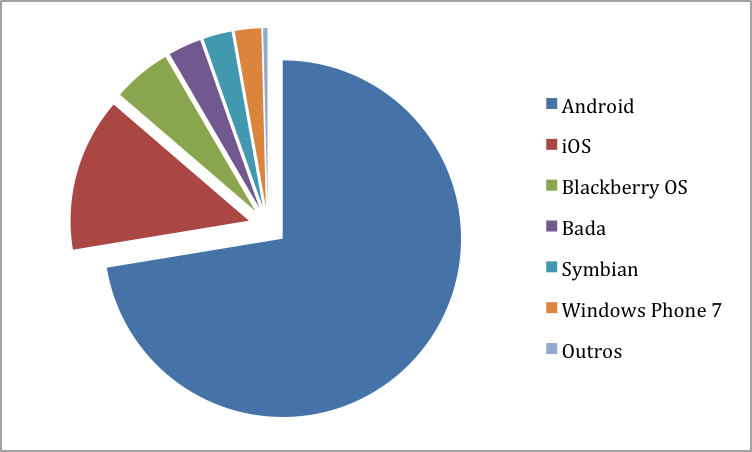
\includegraphics{figs/smartpizza.png}\\
   \caption{ MarketShare Q3 2012}
   \label{FIG:smartpizza}
 \end{figure}
 Fonte: \cite{neowin}
 
 Notadamente, o Android e o iOS s�o as plataformas mais populares. O grande diferencial entre o marketshare desses dois sistemas s�o o segmento de mercado: enquanto o Android atua em todos os segmentos, desde celulares \emph{low-end} aos celulares de ponta, o iOS atua somente com celulares de ponta, chamados \emph{high-end}. Outro fato a considerar � que, nesse gr�fico, n�o s�o considerados outros dispositivos, como tocadores de m�sica e \emph{tablets}.

 \section{iOS}
 \subsection{Vis�o Geral}

 O iOS � um sistema operacional para dispositivos m�veis, lan�ado pela Apple em 2007. Inicialmente, foi desenvolvido para o iPhone, sendo posteriormente aproveitado nos dispositivos iPod Touch, iPad e Apple TV. Ele � um sistema operacional licenciado para rodar apenas em hardware produzido pela Apple, otimizado para a arquitetura de processadores ARM.
 
 Sua entrada de dados � feita de forma direta, atrav�s de multi- toques. Esses toques podem ser desde encostar o dedo, similar a um clique do mouse, at� balan�ar o aparelho, de modo a utilizar seu aceler�metro. Todos os controles de entrada de dados s�o controlados pela \ac{GUI} Cocoa Touch.
 
 O livro \cite{usecabecaiphone} cita que o iPhone revolucionou a maneira de ver um celular: ele �, atualmente, uma plataforma de jogos, um organizador pessoal, um navegador (browser) completo e, claro, um celular. Muito de seu sucesso deve-se ao sucesso da loja virtual ``App Store'', de m�dias e aplicativos, que abriu oportunidade para desenvolvedores independentes competirem em escala mundial com grandes empresas de software. 

 \subsection{Linguagem: Objective-c}
 A programa��o nativa em iOS utiliza uma linguagem de programa��o chamada Objective-C, com o \emph{framework} Foundation. 
 
 O Objective-C � uma linguagem de programa��o reflexiva e orientada a objeto, com origens no SmallTalk e no C. Foi criada no in�cio da d�cada de 80 por Brad Cox e Tom Love, mas somente se tornou popular quando foi licenciada pela NeXT, de Steve Jobs, em 1988. Atualmente � a principal linguagem utilizada para desenvolvimento para Mac OS X.
 
 Como o Objective-C foi construido sobre C, qualquer c�digo C pode ser compilado com um compilador Objective-C. Por defini��o, � uma camada sobre o C que aceita orienta��o a objetos, atrav�s de mensagens.
 
 Em linguagens com ``message parsing'', m�todos n�o s�o chamados de objetos, mas sim mensagens s�o enviadas ao objeto. Essa diferen�a implica em como o c�digo referenciado pelo m�todo ou nome da mensagem � executado. Em nosso caso, o ``alvo'' da mensagem � resolvido em tempo de execu��o, com o objeto receptor interpretando a mensagem.

 \subsection{Ciclo de vida}
 O ciclo de vida constitui uma sequ�ncia de eventos entre o in�cio e a finaliza��o da aplica��o. Um aplicativo iOS come�a quando o usu�rio toca o �cone da mesma na home do dispositivo. Feito isso, o sistema operacional inicia alguns procedimentos de renderiza��o e chama a fun��o principal (main.m) do aplicativo.
 
 Uma vez iniciado, o comando da execu��o passa a ser do UIKit, framework de controle do iOS, que carrega a interface gr�fica e l� o loop de eventos. Durante o loop, o UIKit delega cada evento a seu respectivo objeto e responde aos comandos emitidos pelo aplicativo. Quando o usu�rio realiza uma a��o que causa um evento de sa�da, o UIKit notifica a aplica��o e inicia o processo de sa�da.


 \section{Android}

 \subsection{Vis�o Geral}
 	O Android � a resposta do Google para ocupar o segmento de mercado de sistemas operacionais para plataformas m�veis. Consiste em um novo sistema baseado no sistema operacional Linux, com diversas aplica��es j� instaladas, al�m de um ambiente de desenvolvimento forte e flex�vel. 
	
 	De acordo com \cite{lecheta}, o Android causou um grande impacto quando foi anunciado, em especial pelas empresas que estavam por tr�s de seu desenvolvimento: Google, Motorola, LG, Samsung, Sony, entre muitas outras. A esse grupo de empresas, denominado \ac{OHA}, coube � padroniza��o de uma plataforma de c�digo aberto e livre para celulares, com o objetivo de atender a demanda do mercado atual.
	
 	Um dos pontos fortes do Android � seu sistema flex�vel: � f�cil integrar aplica��es nativas com a sua aplica��o, ou at� mesmo substituir algumas dessas aplica��es nativas pela sua pr�pria. Isso gera um grande apelo para empresas de telefonia, que podem usar dessa personaliza��o para lan�arem suas pr�prias vers�es de aparelhos Android personalizados.
	
 	O grande foco do sistema � a intera��o entre aplicativos: agenda, maps, contatos s�o facilmente alcan��veis por qualquer aplica��o. Essa funcionalidade � realizada por um recurso chamado Intent.%, que ser� abordado em cap�tulos posteriores.
	
 	Outro ponto forte do Android � que seu sistema operacional � baseado no Linux (baseado no kernel 2.6), ou seja, ele mesmo se encarrega de gerenciar a memoria em uso e os processos. Isso faz com que seja poss�vel rodar mais de uma aplica��o (genuinamente) ao mesmo tempo, fazendo com que outros aplicativos rodem em segundo plano durante outros servi�os, como ao atender um telefonema ou acessar a internet.  
	
 	O que � dito como vantagem tamb�m � apontado, fatalmente, como um problema: uma vez que aplicativos podem rodar em segundo plano, aplicativos maliciosos tamb�m podem ser rodados em segundo plano. Durante muito tempo, aplicativos desse tipo podiam ser encontrados para download no Android Market (atualmente Google Play), havendo hoje uma melhor sele��o dos aplicativos que de fato est�o sendo disponibilizados na loja.

 \subsection{Linguagem: Java} 
 	A linguagem nativa de programa��o para Android � o Java, utilizando o framework Android criado pela Open Handset Alliance (OHA).
 	O Java � uma linguagem de prop�sito geral, concorrente e orientada a objetos. Sua primeira vers�o foi lan�ada em 1995 pela Sun Microsystems e, atualmente, encontra-se em sua s�tima vers�o, sendo mantida pela Oracle. 
	
 	Atualmente, � uma das linguagens de programa��o mais populares do mundo, ocupando o 2� lugar no �ndice TIOBE. Devido a isso, h� um grande n�mero de desenvolvedores que possuem o pr�-requisito b�sico para iniciar programa��o para Android: o dom�nio da linguagem.
	
 	O grande sucesso do Java � normalmente creditado a sua capacidade de funcionar nos mais diversos ambientes, desde micro-sistemas como cart�es de cr�dito a grandes plataformas web. Isso � devido a implementa��o de sua m�quina virtual, que � capaz de rodar nas mais diversas plataformas. 


 \subsection{Ciclo de vida}
 	 O ciclo de vida de uma aplica��o Android � controlado por uma Activity, a qual tamb�m gerencia a interface com o usu�rio, recebe requisi��es, realiza o tratamento e processa.
	 
 	Toda Activity possui os seguintes m�todos de controle, a saber:
 \begin{itemize}
 \item onCreate(): � o primeiro m�todo a ser executado em uma Activity. Usualmente � o m�todo respons�vel por carregar os layouts XML e inicializar atributos de classe e outros servi�os.
 \item onStart(): � chamado imediatamente chamado ap�s o onCreate(). Diferentemente deste, � chamado toda vez que a Activity volta a ter foco ap�s um per�odo em background.
 \item onResume(): Assim como o onStart(), � chamado no in�cio da Activity e, tamb�m, quando a mesma volta a ter foco. A diferen�a entre ambos � que o onStart() s� � invocado quando a Activity n�o est� mais vis�vel, enquanto o onResume() � chamado toda vez que retorna o foco.
 \item onPause(): � a primeira fun��o a ser chamada quando a Activity perde o foco.
 \item onStop(): � chamado quando uma Activity � substitu�da por outra Activity
 \item onDestroy(): � o �ltimo m�todo a ser executado. Quando o onDestroy() � executado, a Activity � considerada ``morta'' e fica pronta para ser removida pelo Garbage Collector.
 \item	onRestart(): Chamado quando a Activity sai do estado de ``stop''; ap�s sua execu��o, � chamado o m�todo onStart().
 \end{itemize}

 \section{Redes Sociais}  ser� que vale mesmo a pena falar sobre isso?
 \section{Resumo do Cap�tulo}

 	Neste cap�tulo foram abordadas as tr�s principais tecnologias necess�rias para o desenvolvimento deste projeto: computa��o em nuvem, web services e computa��o m�vel. Tais tecnologias foram aprofundadas em um n�vel o qual fornecessem ao leitor os pr�-requisitos para a compreens�o do restante do projeto, o qual ser� apresentado nos cap�tulos posteriores.
 
%\pdfbookmark[1]
\begin{acronym}

% Meus
\acro {CSS}{\emph{Cascading Style Sheets}}
\acro {DRY}{\emph{don't repeat yourself}}
\acro {GUI}{\emph{Graphic User Interface}}
\acro {HTML}{\emph{HyperText Markup Language}}
\acro {HTTP}{\emph{Hypertext Transfer Protocol}}
\acro {JSON}{\emph{JavaScript Object Notation}}
\acro {JVM}{\emph{Java Virtual Machine}}
\acro {IDE}{\emph{Integrated Development Environment}}
\acro {MVC}{\emph{Model View Controller}}
\acro {NFC}{\emph{Near Field Communication}}
\acro {NIST}{\emph{National Institute of Standarts and Technology}}
\acro {OHA}{\emph{Open Handset Alliance}}
\acro {PaaS}{\emph{Platform as a Service}}
\acro {REST}{\emph{Representational State Transfer}}
\acro {SGBD}{\emph{Sistema de Gerenciamento de Banco de Dados}}
\acro {SOAP}{\emph{Simple Object Access Protocol}}
\acro {SSH}{\emph{Secure Shell}}
\acro {TDD}{\emph{Test Driven Development}}
\acro {URL}{\emph{Uniform Resource Locator}}
\acro {XML}{\emph{Extensible Markup Language}}
\acro {YAML}{\emph{YAML Ain't Markup Language}}
\acro {YARV}{\emph{Yet Another Ruby VM}}

\end{acronym} 
    %\LTXtable{\textwidth}{pretexto/siglas}%%
    %GATHER{pretexto/simbolos.tex}%%
    %GATHER{pretexto/siglas.tex}%%
\end{singlespace}

\pagestyle{capitulo} \setlength{\parskip}{1ex plus 0.5ex}
%%%%%%%%%%%%%%%%%%%%%%%%%%%%%%%%%%%%%%%%%%%%%%%%%%%%%%%%%%%%%%%%
%%% CAP�TULO 1: INTRODU��O
\mainmatter
\chapter{Introdu��o} \label{CHP:INTRO}

\section{Motiva��o}

\section{Objetivos}

Os objetivos gerais e espec�ficos desta monografia, s�o apresentados a seguir.

\subsection{Objetivos Gerais}

\subsection{Objetivos Espec�ficos}



\section{Organiza��o do Texto}





%%%%%%%%%%%%%%%%%%%%%%%%%%%%%%%%%%%%%%%%%%%%%%%%%%%%%%%%%%%%%%%
%%%% CAP�TULO 2: Server-Side
\chapter{Fundamenta��o Te�rica} \label{CHP:FUND}

\section{Servi�os PaaS}
\subsection{Defini��o}

Segundo o \ac{NIST}, o termo computa��o em n�vem tem a seguinte defini��o: ``Cloud Computing (pt: computa��o em nuvem) � um modelo que permite, de forma conveniente, o acesso � rede sob demanda para um conjunto compartilhado de recursos de computa��o configur�veis (por exemplo, redes, servidores, armazenamento, aplicativos e servi�os) que podem ser rapidamente provisionados e lan�ados  com o m�nimo de esfor�o de gest�o ou a intera��o de um prestador de servi�os.''. Um dos servi�os definidos � o \ac{PaaS}.

	Ainda de acordo com o \ac{NIST}, o \ac{PaaS} � ``a capacidade fornecida ao consumidor de publicar aplica��es usando linguagem de programa��o, bibliotecas, servi�os suportados pelo provedor''. Com o fornecimento de tal servi�o, o consumidor n�o precisa se preocupar com o controle de certos servi�os de infra-estrutura, como a rede, servidores, sistemas operacionais, armazenamento, ou seja, criam uma camada de abstra��o de servi�os de infra-estrutura.
	
	De acordo com \cite{cloudstack}, servi�os \ac{PaaS} possuem as seguintes caracter�sticas:
\begin{itemize}
\item Servi�os para desenvolver, testar, publicar, hospedar e manter aplica��es de forma integrada;
\item Arquitetura Multi-tenant, onde v�rios usu�rios podem utilizar o mesmo ambiente de desenvolvimento;
\item Constru��o garantindo escalabilidade, incluindo balanceamento de carga (load balancing) e replica��o de dados para recupera��o de falhas (failover);
\item Integra��o com web services e banco de dados atrav�s de padr�es comuns;
\item Suporte para desenvolvimento em equipes, podendo ter ferramentas de planejamento de projetos e de comunica��o;
\item Ferramentas para gerenciamento dos custos.
\end{itemize}

	Ou seja, sistemas \ac{PaaS} s�o �teis para desenvolvedores individuais e startups\footnote{Termo utilizado para designar modelo de n�gocios repet�vel e escal�vel, em um ambiente de extrema incerteza. Normalmente, projetos ou empresas startups est�o associadas as �reas de tecnologia.}, pois fornecem facilidade de publica��o sem os custos e complexidades de hardwares e softwares inerentes a uma aplica��o web comum \cite{guardianstartup}.
	
\subsection{Heroku}

	O \emph{Heroku} � uma plataforma cloud de servi�os \ac{PaaS} montado sobre o \emph{Amazon EC2}, existente desde junho de 2007. Possui suporte para as seguintes linguagens: Ruby, Java, Node.JS, Scala, Clojure, Python e PHP. Internamente, funciona sobre o sistema operacional Ubuntu.

	Inicialmente, o \emph{Heroku} foi desenvolvido com suporte exclusivo para a linguagem Ruby. Em julho de 2011, Matz Matsumoto, criador do Ruby, entrou para a empresa como Arquiteto-chefe e, nesse mesmo m�s, passou a dar suporte tamb�m para Node.js e Clojure.
Em setembro de 2011, a rede social \emph{Facebook} fez uma parceria com o \emph{Heroku} a fim de facilitar a publica��o de aplicativos para sua pr�pria plataforma \cite{faceheroku}. Em poucos passos, � poss�vel criar uma aplica��o no Facebook e no Heroku, simultaneamente.
O \emph{Heroku} usa uma unidade de m�quina virtual chamada ``Dyno'' com 4 cores e at� 512mb de RAM.

	

\section{REST}
 O \ac{REST} foi definido em uma tese de doutorado por Roy Fielding da seguinte maneira: 
``O REST  � pretendido como uma imagem do design da aplica��o se comportar�: uma rede de websites (um estado virtual), onde o usu�rio progride com uma aplica��o selecionando as liga��es (transi��es do estado), tendo como resultado a p�gina seguinte (que representa o estado seguinte da aplica��o) que est� sendo transferida ao usu�rio e apresentada para seu uso.''

	De modo geral, o \ac{REST} � uma interface de comunica��o onde h� um provedor de servi�os e um consumidor. Tal interface pode ser descrita utilizando \ac{XML}, \ac{HTTP}, \ac{YAML}, \ac{JSON} ou at� mesmo texto puro, de modo a n�o utilizar trocas de mensagens complexas como o \ac{SOAP}. 

O \ac{REST} possui alguns princ�pios, a saber:
\begin{itemize}
\item Modelo provedor/consumidor Stateless (sem estado): cada mensagem \ac{HTTP} trocada possui todas as informa��es necess�rias para a comunica��o, ou seja, nenhuma das partes necessita gravar estado da comunica��o. Em sistemas web, � comum o uso de cookies para manter o estado da sess�o; j� em sistemas mobile, � comum utilizarmos um token de autentica��o, com a mesma finalidade.

\item Opera��es \ac{HTTP}: de modo a diminuir o tr�fego de dados, s�o utilizados m�todos \ac{HTTP} para acessar os recursos de informa��o. As opera��es mais utilizadas s�o o GET, PUT, POST e DELETE. Em sistemas \ac{REST}, � comum combinar tais m�todos com opera��es de CRUD (create, read, update e delete), que faz persist�ncia de dados em um determinado recurso ou entidade.

\item Identifica��o de recursos: As URLs identificam cada uma das entidades e seus elementos, ficando a cargo da opera��o \ac{HTTP} definir a a��o a ser feita com cada um dos recursos ou elementos.

\item Uso de hiperm�dia: As trocas de mensagem de comunica��o � feita utilizando, no corpo da mensagem \ac{HTTP}, uma linguagem de marca��o, conforme j� citado anteriormente. Por�m, n�o h� uma restri��o geral quanto ao uso, podendo ser usada linguagens pr�prias (texto puro).

\end{itemize}
\subsection{RESTful}

	Em uma arquitetura julgada como \emph{RESTful}, o m�todo desejado � informado dentro do m�todo \ac{HTTP}, contido no header do mesmo. Al�m disso, o escopo da informa��o � colocado na \ac{URL}, o que torna uma ``combina��o poderosa''. Por defini��o, uma aplica��o deixa de ser RESTFul caso o m�todo \ac{HTTP} n�o combine com o m�todo da informa��o, ou seja, com a funcionalidade esperada para aquela estrutura de dados. \cite{restfulws}

\section{JSON}
\subsection{Introdu��o}
\ac{JSON} � um padr�o aberto de texto para representar estruturas de dados, de forma intelig�vel para humanos.  Sua origem � a linguagem javascript, e seu formato est� descrtio no RFC 4627.

\subsection{Defini��o}
	O \ac{JSON} � um dos formatos mais usados na serializa��o e transmiss�o de dados estruturados pela internet,ao lado do \ac{XML} e \ac{YAML}, sendo muito usado em sistemas orientados a servi�o / webservice. Muitas linguagens e frameworks, como o Foundation (iOS) e o Android, d�o suporte para esse padr�o, atrav�s de parsers para constru��o e consumo.
De acordo com \cite{restfulws}, ``� muito mais f�cil para um browser lidar com uma estrutura javascript oriunda de uma estrutura JSON do que a partir de um documento XML''. Ainda de acordo com a fonte, cada web browser oferece uma interface JavaScript diferente para seus parsers XML, enquanto um objeto \ac{JSON}, que por defini��o � um objeto JavaScript, ser� interpretado da mesma maneira em qualquer interpretador JavaScript. O \ac{JSON} � uma alternativa mais leve para serializa��o de dados do que o \ac{XML}, definido pelo \ac{XML} Schema. 

\subsection{compara��o com XML}
	\ac{JSON} e \ac{XML} s�o dois formatos de manipula��o de informa��es que podem ser usados com o mesmo objetivo, mas possuem implementa��es e aplica��es distintas. 

	No artigo \cite{comparexmljson}, � feito um estudo considerando a hip�tese de que n�o h� diferen�a em rela��o ao tempo de transmiss�o e os recursos utilizados entre \ac{JSON} e XML.A fim de realizar o estudo, foi criado um ambiente operacional consistindo de uma aplica��o cliente/servidor em Java, onde o servidor escuta uma porta e o cliente conecta a ela. 

	No referido teste, foram utilizadas as seguintes m�tricas: n�mero de objetos enviados, tempo total para enviar o n�mero de objetos, tempo m�dio de transmiss�o, uso da CPU pelo usu�rio, uso da CPU pelo sistema e o uso de mem�ria.

	De acordo com a conclus�o do artigo, codifica��o \ac{JSON} �, em geral, mais r�pida e consome menos recursos que a codifica��o XML, o que nega a hip�tese de igualdade de escolha entre as duas tecnologias. Ou seja, em um ambiente onde � necess�ria velocidade e os recursos s�o limitados, como sistemas m�veis, � prefer�vel utilizar \ac{JSON}.

\subsection{Estrutura}
	De acordo com W3resource \cite{w3json}, o \ac{JSON} suporta duas grandes estruturas de informa��o: cole��o de pares chave/valor e listas ordenadas de valores. Ambas estruturas s�o tamb�m suportadas pela maioria das linguagens de programa��o modernas, o que refor�a a ideia de ser uma boa escolha de linguagem para transmiss�o de informa��es.
	
	O \ac{JSON}possui alguns tipos de dados, a saber:
\begin{itemize}
\item Objetos: um objeto come�a e termina com '{' e '}', contendo um n�mero de pares chave/valor.  A separa��o entre uma chave e um valor � feita com o caractere ':',  e a separa��o entre pares � feita com ','. O valor de um par pode ser qualquer estrutura JSON.
\item Arrays: Um array come�a e termina com '[' e ']'. Entre eles, s�o adicionados certo numero de valores, separados por ','. 
\item Valores: os valores podem ser string, numero, objeto, array, valor booleano ou null.
\end{itemize}
Exemplo de c�digo JSON:

\begin{lstlisting}
{
    "firstName": "Bidhan",
"lastName": "Chatterjee",
    "age": 40,
    "address": {
        "streetAddress": "144 J B Hazra Road",
        "city": "Burdwan",
        "state": "Paschimbanga",
        "postalCode": "713102"
    },
    "phoneNumber": [
        {
            "type": "personal",
            "number": "09832209761"
        },
        {
            "type": "fax",
            "number": "91-342-2567692"
        }
    ]
}
\end{lstlisting}

\section{Ruby on Rails}

\subsection{Ruby}
	Ruby � uma linguagem orientada a objetos, com tipagem forte e din�mica, criada por Yukihiro Matsumoto (Matz) em 1995. 
	
	Segundo \cite{caelum}, uma de suas principais caracter�sticas � sua expressividade, ou seja, a facilidade de ser lida e entendida, o que facilitaria o desenvolvimento de sistemas escritos por ela.
	
	O livro \cite{rails3} lista algumas das caracter�sticas mais importantes do Ruby, a saber:
\begin{itemize}
\item � uma linguagem interpretada, ou seja, um interpretador l� o c�digo e decide como executar em tempo de execu��o. Por consequ�ncia, um sistema em Ruby pode se tornar um pouco mais lento, por�m, � not�vel o ganho em flexibilidade.
\item Possui uma sintaxe de linguagem flex�vel, fazendo com que a curva de aprendizado seja menor em rela��o a outras linguagens. Um exemplo cl�ssico � a n�o-necessidade (opcional) de escrever par�nteses ao redor dos par�metros de um m�todo. Entretanto, podem surgir erros misteriosos por n�o colocar par�nteses em algumas situa��es amb�guas.
\item Possui uma tipagem din�mica, ou seja, n�o � necess�rio especificar o tipo de informa��o que ser� guardado em cada vari�vel. Isso torna a abordagem bem mais flex�vel, tornando as opera��es dependentes do pr�prio contexto. Entretanto, problemas podem ocorrer justamente por isso: comportamentos inesperados.
\item Suporte a blocos e closures,
\end{itemize}
	
	Atualmente, Ruby encontra-se entre as linguagens de programa��o mais populares, ocupando a posi��o 11� no �ndice Tiobe\footnote{O �ndice TIOBE mede, mensalmente, a popularidade de uma determinada linguagem de programa��o, baseado no numero de engenheiros qualificados, cursos, vendedores e buscas nos principais motores de busca. Pode ser encontrado em \url{http://www.tiobe.com/index.php/content/paperinfo/tpci/index.html} }.  Grande parte desse sucesso deve-se ao framework Rails, implementado como solu��o web utilizando Ruby.

\subsection{Rails}
	O Ruby on Rails, tamb�m chamado Rails ou RoR, � um framework de desenvolvimento web de c�digo aberto que tem como premissa aumentar a velocidade e a facilidade no desenvolvimento de aplica��es web orientados a banco de dados.  Foi lan�ado oficialmente em Julho de 2004 pelo seu criador David H. Hansson, estando atualmente na vers�o 3.2.11, com a 4� vers�o em desenvolvimento \cite{rails4}.  
	
	O Rails � um framework full-stack, ou em portugu�s, pilha completa. Isso significa que, com ele, � poss�vel desenvolver a aplica��o por completo, desde o desenvolvimento dos layouts das paginas, a manuten��o do banco de dados. Al�m disso, o Rails enfatiza o uso de alguns padr�es de engenharia de software, a saber:
	
\begin{itemize}
\item Active record: padr�o de projeto para armazenamento de dados em banco de dados relacionais.  A interface de um certo objeto deve incluir fun��es de CRUD,  como inserir, atualizar, apagar e algumas fun��es de consulta. Cada tabela de um banco de dados � embrulhada (wrapped) em um uma classe, sendo cada instancia dessa classe um registro (tupla) �nico na tabela.  Esse conceito est� definido em \cite{fowler}.
\item Conven��o sobre configura��o: modelo de desenvolvimento de software que busca diminuir o n�mero de decis�es que os desenvolvedores precisam tomar, ou seja, o desenvolvedor n�o precisa definir aspectos convencionais da aplica��o. Em Rails, � f�cil perceber esse padr�o na escolha dos nomes das tabelas: se um modelo chama-se ``Usuario'', a tabela correspondente se chamar� ``Usuarios'' e, se existir uma rela��o entre usu�rios e contas (m:m), a nova tabela ser� denominada, automaticamente, $usuarios_contas$.
\item \ac{DRY}: O objetivo principal � reduzir a repeti��o de informa��o de qualquer tipo. Esse conceito incentiva o bom uso da reutiliza��o de c�digo, que � tamb�m uma das principais vantagens da orienta��o a objetos.
\item \ac{MVC}: esse padr�o de arquitetura de software separa a aplica��o em tr�s camadas: uma contendo a l�gica da aplica��o e regra de neg�cios, chamada model; uma contendo a entrada e sa�da de dados com o usu�rio, chamada view; uma interligando ambas, de maneira a manipular dados da view para o model entender e vice-versa, chamada controller. O principal objetivo dessa arquitetura � a reusabilidade de c�digo e a separa��o de conceitos \cite{mvc}.
\end{itemize}


 	De acordo com \cite{caelum}, a estrutura a qual o Rails � feito permite que as funcionalidades de um sistema possam ser implementadas de maneira incremental, por conta dos padr�es e conceitos supracitados. Por conseq��ncia, isso tornaria o Rails uma boa escolha para projetos e empresas que adotam metodologias �geis no desenvolvimento da aplica��o.

 	O Ruby � uma linguagem interpretada. Antes de se tornar popular, existia apenas um interpretador dispon�vel, escrito em C pelo pr�prio criador da linguagem. Hoje em dia, o interpretador mais conhecido � o 1.9 ou YARV (Yet Another Ruby VM), para a vers�o mais atualizada e est�vel (Ruby 1.9.3.).
 	
	Existem outros interpretadores Ruby famosos, como:
 \begin{itemize}
 \item JRuby: implementa��o alternativa que permite usar a \ac{JVM} do Java para interpetar c�digo Ruby. Uma de suas principais vantagens � a interoperabilidade com c�digo Java existente, al�m de aproveitar as vantagens j� maduras do java: garbage collector, threas nativas, etc.
 \item IronRuby: Implementa��o .Net da linguagem, mantido pela pr�pria Microsoft
 \item Rubinius: Traz id�ias de m�quinas virtuais do SmallTalk e � implementada em C/C++.
 \end{itemize}
 \section{Smartphones}

 	O mercado de smartphones est� crescendo cada vez mais. Estima-se que no �nicio de 2012 o n�mero de celulares inteligentes tenha atingido a marca de 1 bilh�o de unidades vendidas e, segundo proje��es, esse n�mero deve dobrar em 2015 \cite{yahoosmart}. 
 	
	Embora o n�mero de smartphones seja expressivo, ele ainda � pequeno se comparado ao n�mero de pessoas que possuem um aparelho celular: 3 bilh�es. Isso significa que ainda h� muito espa�o para crescimento, em particular em mercados emergentes como a China, �ndia e �frica.
 	
	Usualmente, um smartphone possui alguns recursos de ponta, como c�mera, bom reprodutor de m�dia, bom processamento gr�fico para jogos, bluetooth, GPS, acesso a internet via wi-fi e 3G/4G, \ac{NFC}, um bom sistema operacional, entre outros. 
 Atualmente, os sistemas operacionais mais populares para smartphones s�o: Android, iOS (Apple), Blackberry OS (RIM), Bada (Samsung), Symbian e Windows Phone 7 (Microsoft). A distribui��o do mercado, no Q3 de 2012, pode ser vista no seguinte gr�fico:
 \begin{figure}[H]
   % Requires \usepackage{graphicx}
   \centering
   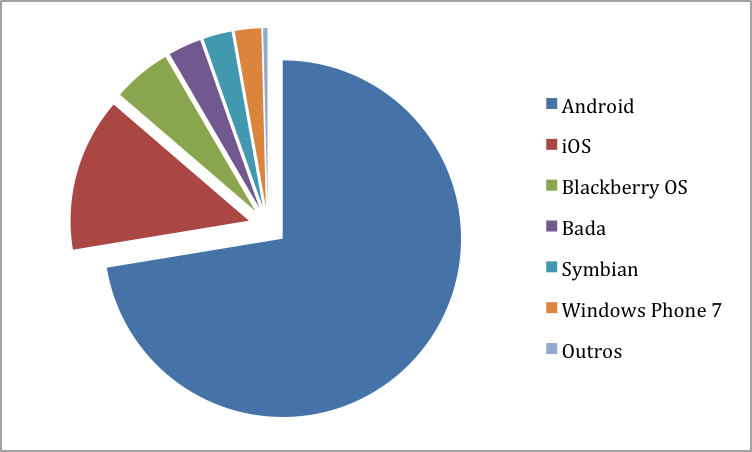
\includegraphics{figs/smartpizza.png}\\
   \caption{ MarketShare Q3 2012}
   \label{FIG:smartpizza}
 \end{figure}
 Fonte: \cite{neowin}
 
 Notadamente, o Android e o iOS s�o as plataformas mais populares. O grande diferencial entre o marketshare desses dois sistemas s�o o segmento de mercado: enquanto o Android atua em todos os segmentos, desde celulares \emph{low-end} aos celulares de ponta, o iOS atua somente com celulares de ponta, chamados \emph{high-end}. Outro fato a considerar � que, nesse gr�fico, n�o s�o considerados outros dispositivos, como tocadores de m�sica e \emph{tablets}.

 \section{iOS}
 \subsection{Vis�o Geral}

 O iOS � um sistema operacional para dispositivos m�veis, lan�ado pela Apple em 2007. Inicialmente, foi desenvolvido para o iPhone, sendo posteriormente aproveitado nos dispositivos iPod Touch, iPad e Apple TV. Ele � um sistema operacional licenciado para rodar apenas em hardware produzido pela Apple, otimizado para a arquitetura de processadores ARM.
 
 Sua entrada de dados � feita de forma direta, atrav�s de multi- toques. Esses toques podem ser desde encostar o dedo, similar a um clique do mouse, at� balan�ar o aparelho, de modo a utilizar seu aceler�metro. Todos os controles de entrada de dados s�o controlados pela \ac{GUI} Cocoa Touch.
 
 O livro \cite{usecabecaiphone} cita que o iPhone revolucionou a maneira de ver um celular: ele �, atualmente, uma plataforma de jogos, um organizador pessoal, um navegador (browser) completo e, claro, um celular. Muito de seu sucesso deve-se ao sucesso da loja virtual ``App Store'', de m�dias e aplicativos, que abriu oportunidade para desenvolvedores independentes competirem em escala mundial com grandes empresas de software. 

 \subsection{Linguagem: Objective-c}
 A programa��o nativa em iOS utiliza uma linguagem de programa��o chamada Objective-C, com o \emph{framework} Foundation. 
 
 O Objective-C � uma linguagem de programa��o reflexiva e orientada a objeto, com origens no SmallTalk e no C. Foi criada no in�cio da d�cada de 80 por Brad Cox e Tom Love, mas somente se tornou popular quando foi licenciada pela NeXT, de Steve Jobs, em 1988. Atualmente � a principal linguagem utilizada para desenvolvimento para Mac OS X.
 
 Como o Objective-C foi construido sobre C, qualquer c�digo C pode ser compilado com um compilador Objective-C. Por defini��o, � uma camada sobre o C que aceita orienta��o a objetos, atrav�s de mensagens.
 
 Em linguagens com ``message parsing'', m�todos n�o s�o chamados de objetos, mas sim mensagens s�o enviadas ao objeto. Essa diferen�a implica em como o c�digo referenciado pelo m�todo ou nome da mensagem � executado. Em nosso caso, o ``alvo'' da mensagem � resolvido em tempo de execu��o, com o objeto receptor interpretando a mensagem.

 \subsection{Ciclo de vida}
 O ciclo de vida constitui uma sequ�ncia de eventos entre o in�cio e a finaliza��o da aplica��o. Um aplicativo iOS come�a quando o usu�rio toca o �cone da mesma na home do dispositivo. Feito isso, o sistema operacional inicia alguns procedimentos de renderiza��o e chama a fun��o principal (main.m) do aplicativo.
 
 Uma vez iniciado, o comando da execu��o passa a ser do UIKit, framework de controle do iOS, que carrega a interface gr�fica e l� o loop de eventos. Durante o loop, o UIKit delega cada evento a seu respectivo objeto e responde aos comandos emitidos pelo aplicativo. Quando o usu�rio realiza uma a��o que causa um evento de sa�da, o UIKit notifica a aplica��o e inicia o processo de sa�da.


 \section{Android}

 \subsection{Vis�o Geral}
 	O Android � a resposta do Google para ocupar o segmento de mercado de sistemas operacionais para plataformas m�veis. Consiste em um novo sistema baseado no sistema operacional Linux, com diversas aplica��es j� instaladas, al�m de um ambiente de desenvolvimento forte e flex�vel. 
	
 	De acordo com \cite{lecheta}, o Android causou um grande impacto quando foi anunciado, em especial pelas empresas que estavam por tr�s de seu desenvolvimento: Google, Motorola, LG, Samsung, Sony, entre muitas outras. A esse grupo de empresas, denominado \ac{OHA}, coube � padroniza��o de uma plataforma de c�digo aberto e livre para celulares, com o objetivo de atender a demanda do mercado atual.
	
 	Um dos pontos fortes do Android � seu sistema flex�vel: � f�cil integrar aplica��es nativas com a sua aplica��o, ou at� mesmo substituir algumas dessas aplica��es nativas pela sua pr�pria. Isso gera um grande apelo para empresas de telefonia, que podem usar dessa personaliza��o para lan�arem suas pr�prias vers�es de aparelhos Android personalizados.
	
 	O grande foco do sistema � a intera��o entre aplicativos: agenda, maps, contatos s�o facilmente alcan��veis por qualquer aplica��o. Essa funcionalidade � realizada por um recurso chamado Intent.%, que ser� abordado em cap�tulos posteriores.
	
 	Outro ponto forte do Android � que seu sistema operacional � baseado no Linux (baseado no kernel 2.6), ou seja, ele mesmo se encarrega de gerenciar a memoria em uso e os processos. Isso faz com que seja poss�vel rodar mais de uma aplica��o (genuinamente) ao mesmo tempo, fazendo com que outros aplicativos rodem em segundo plano durante outros servi�os, como ao atender um telefonema ou acessar a internet.  
	
 	O que � dito como vantagem tamb�m � apontado, fatalmente, como um problema: uma vez que aplicativos podem rodar em segundo plano, aplicativos maliciosos tamb�m podem ser rodados em segundo plano. Durante muito tempo, aplicativos desse tipo podiam ser encontrados para download no Android Market (atualmente Google Play), havendo hoje uma melhor sele��o dos aplicativos que de fato est�o sendo disponibilizados na loja.

 \subsection{Linguagem: Java} 
 	A linguagem nativa de programa��o para Android � o Java, utilizando o framework Android criado pela Open Handset Alliance (OHA).
 	O Java � uma linguagem de prop�sito geral, concorrente e orientada a objetos. Sua primeira vers�o foi lan�ada em 1995 pela Sun Microsystems e, atualmente, encontra-se em sua s�tima vers�o, sendo mantida pela Oracle. 
	
 	Atualmente, � uma das linguagens de programa��o mais populares do mundo, ocupando o 2� lugar no �ndice TIOBE. Devido a isso, h� um grande n�mero de desenvolvedores que possuem o pr�-requisito b�sico para iniciar programa��o para Android: o dom�nio da linguagem.
	
 	O grande sucesso do Java � normalmente creditado a sua capacidade de funcionar nos mais diversos ambientes, desde micro-sistemas como cart�es de cr�dito a grandes plataformas web. Isso � devido a implementa��o de sua m�quina virtual, que � capaz de rodar nas mais diversas plataformas. 


 \subsection{Ciclo de vida}
 	 O ciclo de vida de uma aplica��o Android � controlado por uma Activity, a qual tamb�m gerencia a interface com o usu�rio, recebe requisi��es, realiza o tratamento e processa.
	 
 	Toda Activity possui os seguintes m�todos de controle, a saber:
 \begin{itemize}
 \item onCreate(): � o primeiro m�todo a ser executado em uma Activity. Usualmente � o m�todo respons�vel por carregar os layouts XML e inicializar atributos de classe e outros servi�os.
 \item onStart(): � chamado imediatamente chamado ap�s o onCreate(). Diferentemente deste, � chamado toda vez que a Activity volta a ter foco ap�s um per�odo em background.
 \item onResume(): Assim como o onStart(), � chamado no in�cio da Activity e, tamb�m, quando a mesma volta a ter foco. A diferen�a entre ambos � que o onStart() s� � invocado quando a Activity n�o est� mais vis�vel, enquanto o onResume() � chamado toda vez que retorna o foco.
 \item onPause(): � a primeira fun��o a ser chamada quando a Activity perde o foco.
 \item onStop(): � chamado quando uma Activity � substitu�da por outra Activity
 \item onDestroy(): � o �ltimo m�todo a ser executado. Quando o onDestroy() � executado, a Activity � considerada ``morta'' e fica pronta para ser removida pelo Garbage Collector.
 \item	onRestart(): Chamado quando a Activity sai do estado de ``stop''; ap�s sua execu��o, � chamado o m�todo onStart().
 \end{itemize}

 \section{Redes Sociais}  ser� que vale mesmo a pena falar sobre isso?
 \section{Resumo do Cap�tulo}

 	Neste cap�tulo foram abordadas as tr�s principais tecnologias necess�rias para o desenvolvimento deste projeto: computa��o em nuvem, web services e computa��o m�vel. Tais tecnologias foram aprofundadas em um n�vel o qual fornecessem ao leitor os pr�-requisitos para a compreens�o do restante do projeto, o qual ser� apresentado nos cap�tulos posteriores.
 

%%%% CAP�TULO 3: Aplica��o
\chapter{Aplica��o} \label{CHP:TEO}%%

\section{Vis�o geral}
\begin{figure}[H]
  % Requires \usepackage{graphicx}
  \centering
  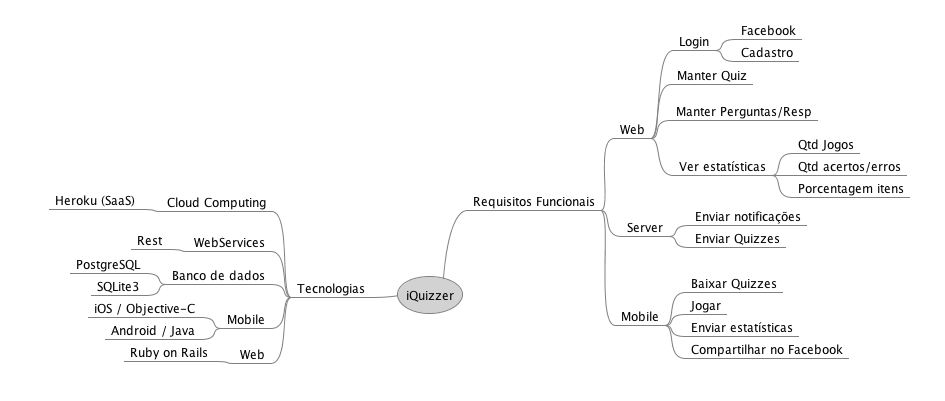
\includegraphics[scale =0.45]{figs/mapa_mental_Quizzer.png}\\
  \caption{ Mapa Mental}
  \label{FIG:Form_Factor0}
\end{figure}
\section{Requisitos}
\subsection{Requisitos funcionais}
\subsection{Requisitos n�o-funcionais}
\section{Casos de uso}
\begin{figure}[H]
  % Requires \usepackage{graphicx}
  \centering
  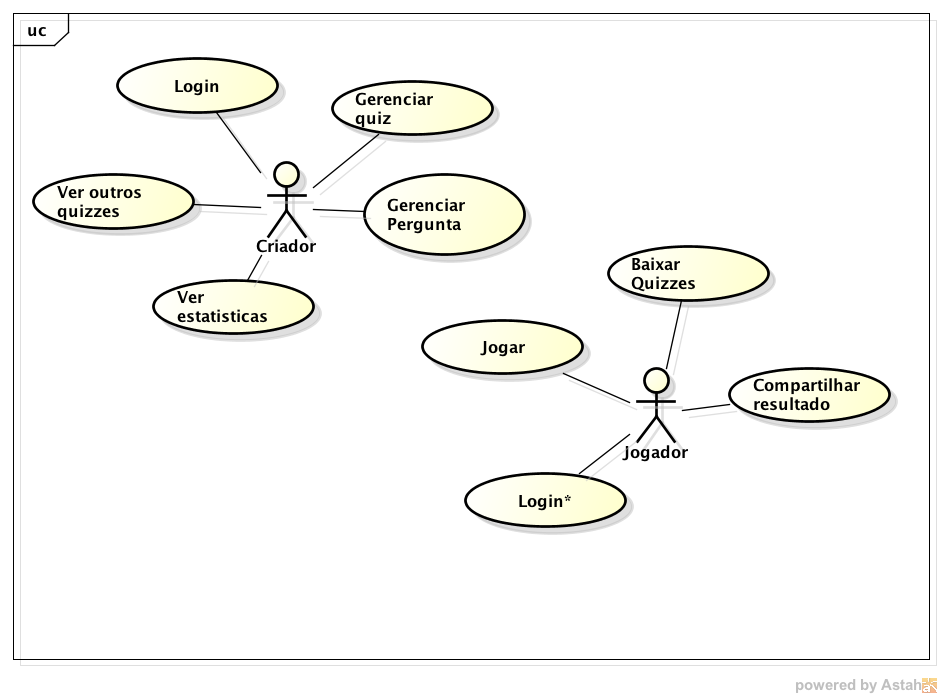
\includegraphics[scale =0.45]{figs/casos_de_uso.png}\\
  \caption{ Diagrama de casos de uso para Criador e Jogador }
  \label{FIG:Form_Factor}
\end{figure}
\section{Diagrama de classes}

\section{Diagrama de entidades}
\begin{figure}[H]
  % Requires \usepackage{graphicx}
  \centering
  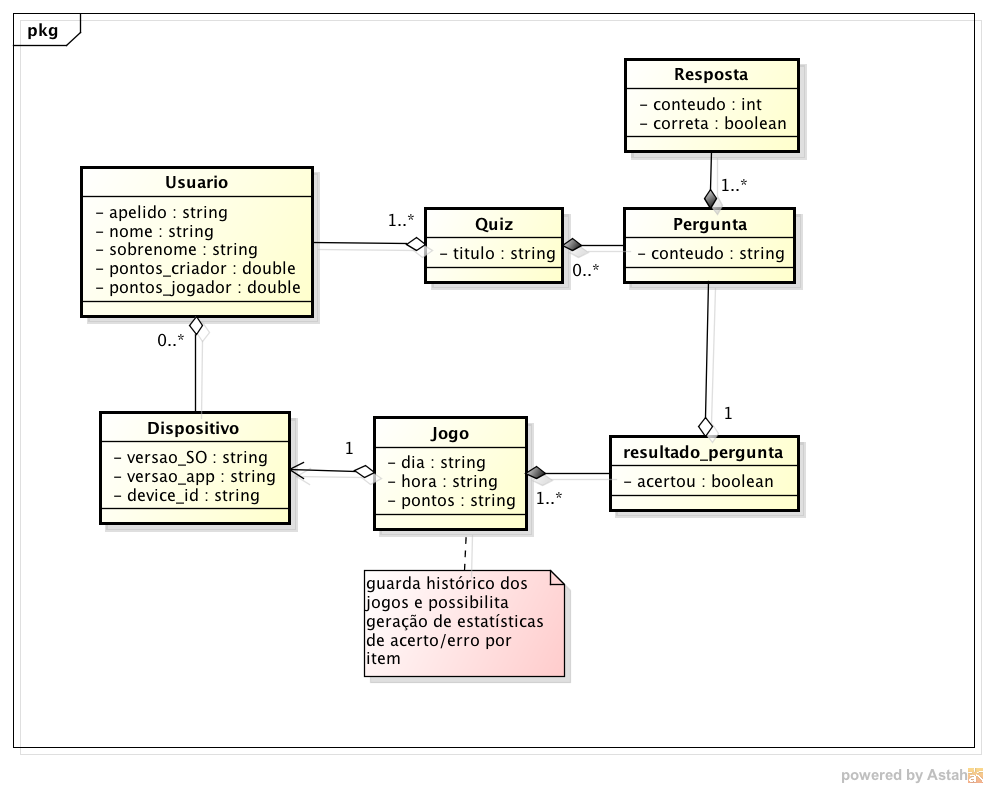
\includegraphics[scale =0.45]{figs/MER_web.png}\\
  \caption{ Diagrama de entidades }
  \label{FIG:Form_Factor2}
\end{figure}
%%%%%%%%%%�%%%%%%%%%%%%%%%%%%%%%%%%%%%%%%%%%%%%%%%%%%%%%%%%%%%%%%%
%%%% CAP�TULO 4: Rails
\chapter{Implementa��o web} \label{CHP:MET}%%
\section{Cria��o de aplica��o}
\section{Rotas}
\section{Autentica��o}
\section{Front-End com bootstrap}
\section{Deploy}
%%%%%%%%%%%%%%%%%%%%%%%%%%%%%%%%%%%%%%%%%%%%%%%%%%%%%%%%%%%%%%%%%
%%%% CAP�TULO 5: iOS
    \chapter{Comparativo Android x iOS} \label{CHP:MET}%%
    \section {Ambienta��o}
     
    iOS
    Para implementa��o nativa de aplica��es, utilizamos a IDE gratuita chamada Xcode. Desenvolvida pela Apple Inc., funciona apenas sobre o sistema operacional Mac OS X.  Por padr�o, j� vem com suporte ao Objective-C, linguagem de programa��o utilizada para desenvolvimento de aplicativos nativos no Mac OS X e no iOS.
    Atualmente, o Xcode est� na vers�o 4.5.2 e pode ser baixado via Mac App Store, de forma gratuita para usu�rios do Mac OS X Lion e OS X Mountain Lion \url{https://itunes.apple.com/us/app/xcode/id497799835}.
    Para desenvolvimento iOS, � necess�rio possuir o iOS SDK, que pode ser baixado internamente a ferramenta Xcode. Entretanto, para realiza��o de testes no dispositivo, � necess�rio a posse da licen�a de desenvolvimento.
     
    Android
            Para o desenvolvimento de aplica��es nativas em Android, necessitamos de um ambiente que possua Android SDK instalado. � poss�vel, por exemplo, gerar aplicativos utilizando apenas um editor de texto, como Notepad ou Gedit. Entretanto, a Google recomenda o uso do Eclipse com ADT Plugin (link).
           
     
    \subsection{IDEs}
    \section {Arquitetura}
    \subsection {Arquivos gerados}
     
     
    \section {Controles b�sicos}
    \subsection {Mostrando textos}
    iOS
    Para exibir textos sem intera��o direta com o usu�rio, utilizamos uma inst�ncia da classe UILabel. Essa classe possui algumas propriedades para modifica��o de aspectos, a saber:
\begin{itemize}
\item text: o texto mostrado no campo;
\item textColor: cor do texto;
\item numberOfLines: n�mero m�ximo de linhas suportadas;
\item font: fonte utilizada pelo texto, inst�ncia de UIFont.
\end{itemize}     
    Android
     
    De maneira similar ao iOS, o Android possui um controle espec�fico para mostrar textos na tela, chamado TextView. Um TextView pode ser definido no layout XML ou no pr�prio Java. Assim como no iOS, possui uma propriedade do tipo String chamada "text", a qual representa o texto apresentado. Possui tamb�m algumas propriedades, a saber:
    [as propriedades legais]
    Uma diferen�a importante entre o UILabel e o TextView � que o �ltimo aceita intera��es com o usu�rio; podemos colocar eventos de intera��o com o usu�rio. Essa funcionalidade costuma ser usada com textos que representam links (URLs).
     
    \subsection {Inserindo textos}
     
    iOS
            Para entrada de textos, utilizamos uma ist�ncia de UITextField. A manipula��o do texto � feita atrav�s do disparo de uma a��o para um ``target'' quando o usu�rio pressiona o bot�o ``return'' do teclado.
    Essa classe normalmente � associada a um UITextFieldDelegate, o qual fornece m�todos adicionais de decis�o.
    Quando o usu�rio toca em um textfield, esse controle torna-se o ``first responder'' e invoca o aparecimento do teclado para o sistema. O teclado deve ser configurado, pelo desenvolvedor, para desaparecer quando o bot�o de return for pressionado. Isso deve ser feito atrav�s da mensagem ``resignFirstResponder'', a ser enviada para o textfield.
    Para que o textfield n�o fique ``escondido'' na tela, embaixo do teclado, cabe ao desenvolvedor mover tela de maneira conveniente, de forma a aparecer o conte�do.
    A apar�ncia do teclado pode ser configurada utilizando o protocolo UITextInputTraits. Existem, entretanto, alguns tipos de teclado a serem definidos por padr�o, como o ASCII, Number, Url, Email, entre outros.
     
    Android
     
    Para a entrada de texto do usu�rio, o Android fornece o controle chamado EditText. Assim como o UITextField, esse controle possui uma propriedade chamada "text", que representa o texto mostrado no controle. Esse texto pode ser tanto a entrada do usu�rio como tamb�m um texto configurado via programa��o pelo aplicativo.
    O EditText possui algumas propriedades que usamos na aplica��o, como as seguintes:
    [propriedades legais]
    Para cada EditText, podemos definir o tipo de teclado que ser� exibido ao interagir com o usu�rio, como teclados de telefone, numeros e de letras.
    O EditText possui duas grandes diferen�as em rela��o ao UITextField, a saber:
\begin{itemize}
\item O teclado retorna automaticamente quando terminada a edi��o;
\item Ao entrar em modo de edi��o, o EditText faz com que a tela do aplicativo desloque-se, caso seja necess�rio para aparecer o conte�do do controle.
\end{itemize}     
     
    \subsection {bot�es e eventos}
     
    iOS
           
    Um bot�o � representando por uma inst�ncia da classe UIButton. Os bot�es interceptam eventos de toque e enviam mensagens para um target pr�-definido quando tocados. M�todos para configurar os targets e a��es s�o herdados de UIControl. Possuem t�tulo, imagem e outras propriedades de apar�ncia.
     
     
    Os bot�es respondem a algumas a��es, como touch drag, touch down, touch up, entre outros. Para associar um m�todo a um evento, criamos uma IBAction (m�todo) e, ao evento, indicamos tal IBAction. Isso pode ser feito facilmente no Interface Builder/Xcode ``ligando'' o bot�o ao c�digo correspondente (file's owner desse bot�o), conforme os passos abaixo:
\begin{enumerate}     
\item Arrastar, com o bot�o direito, o bot�o ao c�digo do file's owner
         
 \item Nomear um IBAction e associar um evento
 \end{enumerate}    
     
    Android
     
    Os bot�es no Android pertencem a classe Button. Existem duas formas de inserir eventos nos bot�es, a saber:
\begin{itemize}
\item via Listener Java: podemos implementar o OnClickListener na Activity ou em alguma classe an�nima dentro da Activity, de modo que ao disparar o evento de click, o m�todo onClick da interface seja chamado.
\item via propriedade onClick no XML: os bot�es possuem uma propriedade chamada onClick, que recebem uma String como valor. Esse valor � o nome do m�todo da Activity onde o layout contendo esse bot�o foi inflado.
    Em nosso projeto, utilizamos somente onClick como propriedade XML, uma vez que toda a parte de layout foi implementada via XML.
\end{itemize}    
    \section {Criando listas}
    iOS
     
    Listas em iOS s�o feitas utilizando inst�ncias de UITableView. Essa classe, por sua vez, estende de UIScrollView, que habilita a rolagem vertical (e apenas a vertical). Internamente, cada linha (c�lula) � representada por um objeto de UITableViewCell, que s�o totalmente configur�veis.
    Esse controle normalmente � associado a um UINavigationController: quando uma c�lula � tocada, � feito um push de um novo UIViewController, detalhando a c�lula.
    Table views possuem dois estilos, a saber: UITableViewStylePlain e UITableViewGrouped. Uma vez criado o controle, n�o � poss�vel mudar o estilo. No estilo Plain, as se��es de header/footer flutuam nas bordas do conte�do. Nesse estilo, pode haver um �ndice variando de A - Z, que facilita a navega��o vertical. No estilo Grouped, uma cor padr�o � definida para o fundo da view e das c�lulas. Nesse estilo, podem ser criadas v�rias listas, de formas agrupadas. Nesse caso, n�o podem ter �ndice.
    Muitos m�todos utilizam o objeto do tipo NSIndexPath como par�metro e retornam valores. Esse objeto representa o �ndice da linha atual e da se��o atual.
    Um objeto do tipo Table View necessita de um objeto que atue como fonte de dados (data source) e um objeto que atue como delegate. Normalmente, utilizamos os protocolos UITableViewDataSource e UITableViewDelegate no UIController no qual o table view esteja inserido. O data source fornece informa��o que o UITableView precisa para construir tabelas e o delegate fornece as c�lulas e executa alguns outros m�todos de manipula��o.
    A fim de criar uma table view b�sica, precisamos implementar, no m�nimo, os seguintes m�todos data source:
\begin{enumerate}
\item N�mero de se��es - retorna o n�mero de se��es para essa table view
  \begin{lstlisting}   
    -(NSInteger)numberOfSectionsInTableView:(UITableView *)tableView
       \end{lstlisting}   
\item N�mero de rows (linhas): retorna o n�mero de linhas para cada uma das se��es
   \begin{lstlisting}  
    - (NSInteger)tableView:(UITableView *)tableView numberOfRowsInSection:
    (NSInteger)section  
        \end{lstlisting}     
\item cell for rows at index: define uma c�lula para cada index (par linha/se��o) da tabela
\begin{lstlisting}    
-(UITableViewCell *)tableView:(UITableView *)tableView cellForRowAtIndexPath:(NSIndexPath *)indexPath
\end{enumerate}     
       \end{lstlisting}
\end{enumerate} 
    Al�m desses m�todos, � comum implementar um m�todo delegate que responda a cada c�lula tocada, como a seguir:
 
    I. did select row at index: informa o par (linha/se��o) que foi selecionado. A partir do index path, pode-se recuperar a c�lula selecionada dentro da table view
\begin{lstlisting}   
    - (NSInteger)tableView:(UITableView *)tableView numberOfRowsInSection:
    (NSInteger)section  
          \end{lstlisting}   
     
    Para a tela de escolha dos quizzes (GameMenu), implementamos uma table view simples, da seguinte maneira:
\begin{lstlisting}   
    -(NSInteger)numberOfSectionsInTableView:(UITableView *)tableView{
    return1;
    }
    -(NSInteger)tableView:(UITableView *)tableView numberOfRowsInSection:(NSInteger)section{
    //conta no array de quizzes a quantidade de elementos
    return [self.quizzescount];
    }
    -(UITableViewCell*)tableView:(UITableView *)tableView cellForRowAtIndexPath:(NSIndexPath *)indexPath{
    //reaproveita ou cria uma c�lula
    UITableViewCell* cell = [tableView dequeueReusableCellWithIdentifier:@"cell"];
    if (cell == nil){
    cell = [[UITableViewCellalloc] init];
    }
     
    //personaliza��o da c�lula
    Quiz* q = [self.quizzesobjectAtIndex:indexPath.row];
    cell.textLabel.text = [q titulo];
    return cell;
    }
    //disparado quando um dos quizzes for selecionado
    -(void)tableView:(UITableView *)tableView didSelectRowAtIndexPath:(NSIndexPath *)indexPath{
    Quiz* q = [self.quizzesobjectAtIndex:indexPath.row];
    GameViewController* gq = [[GameViewControlleralloc] initWithNibName:@"GameViewController"bundle:nil];
    gq.quiz = q;
    NSLog(@"quiz.content: %@",q.titulo);
    NSLog(@"count perguntas: %d", q.perguntas.count);
    [self.navigationControllerpushViewController:gq animated:YES];
    }
            \end{lstlisting} 
    Android
            As listas em Android s�o inst�ncias da classe widget ListView e, assim como no iOS, j� possui rolagem vertical implementada. Os itens da lista s�o inseridos por outra classe controladora, chamada Adapter.
            O Adapter � uma classe que prov� acesso aos itens que cont�m a informa��o, como um array de strings. Al�m disso, o Adapter � respons�vel por criar o layout de cada c�lula.
            Para a lista simples mostrada em GameMenu, foi implementado uma lista com c�lulas padr�o da seguinte maneira:
\begin{lstlisting}   
        private void carregarLista() {
     
         ArrayAdapter arrayAdapter = new ArrayAdapter(this, android.R.layout.simple_list_item_1, quizzes);
       ListView listView = (ListView)findViewById(R.id.lista_quizzes);
    listView.setAdapter(arrayAdapter);
    listView.setOnItemClickListener(this);
     
    }
            \end{lstlisting} 
            Nesse trecho de c�digo, quizzes � um ArrayList de quizzes. ArrayAdapter e ListView s�o classes padr�o do Android.  
    Os eventos de clique de c�lula est�o associados a classe que implementa a interface OnItemClickListener.  Tal interface exige a implementa��o do m�todo onClickListener. Foi utilizado, no iQuizzer, esse listener na classe GameMenu, tendo sido implementado o m�todo da seguinte maneira:
\begin{lstlisting}   
            @Override
    public void onItemClick(AdapterView<?> adapterView, View view, int position, long id) {
    Quiz quiz = quizzes.get(position);
      Intent i = new Intent(getApplicationContext(), GameActivity.class);
      i.putExtra("quiz",quiz);
      startActivity(i);
    }
             \end{lstlisting}    
    \section{Personalizando linhas de uma lista} -- retirado
    iOS
    Android
    \section {Acesso a dados}
     
    \subsection {SQLite}
            O SQLite � uma biblioteca implementada em C, de dom�nio p�blico, que representa um banco de dados SQL. Tem como caracter�sticas fundamentais ser contido em si mesmo, livre de servidores, sem configura��o e transacional. (\url{http://www.sqlite.org/about.html}).
            Tanto o iOS quanto o Android possuem abstra��es para representar objetos da tabela (active records), conex�es e o pr�prio banco.
     
    iOS
            Existem duas maneiras de se trabalhar com SQLite em iOS: acesso nativo atrav�s da biblioteca SQLite.h e Core Data Framework.
            No acesso nativo, a programa��o utilizada � a mesma para aplica��es nativas em C, ou seja, n�o h� particularidades entre utilizar o SQLite dentro ou fora do iOS. J� em Core Data, a programa��o � em Objective-C e existe uma camada de abstra��o do banco de dados.
            Em nossa aplica��o, optamos por usar o Core Data devido � facilidade de fazer a modelagem utilizando o xcdatamodel. O xcdatamodel � uma ferramenta facilitadora, integrada ao Xcode, na qual o desenvolvedor pode ``desenhar'' as tabelas e criar liga��es, chamadas ``relationships''. Cada uma das tabelas e rela��es possuem propriedades, que s�o facilmente configuradas.
     
     
     
            Existem tr�s classes principais de abstra��o de banco de dados, a saber:
\begin{itemize}
\item Managed Object Model: � a classe que cont�m as defini��es de cada objeto (entidades, active record);
\item Persistent store coordinator: � a conex�o do banco; s�o configurados os nomes e a localiza��o da base de dados;
\item Managed Object Context: classe respons�vel pelas opera��es b�sicas de manipula��o: inserir objetos, deletar objetos, etc.
\end{itemize}
    No iQuizzer para iOS, criamos uma classe chamada DAO e implementamos m�todos de CRUD, como pesquisar, inserir, modificar e deletar. Para cada uma das entidades, criamos uma classe de DAO estendida, como QuizDAO ou PerguntaDAO, onde cada uma dessas realiza opera��es de crud mais especificas e voltadas para as situa��es que ocorrem na aplica��o. Nessas classes de DAO, fazemos manipula��o de ``managed object contexto'' e ``persistente store coordinator''.
            Para cada uma das entidades, criamos um managed object model, estendendo da classe nativa NSManagedObject. � poss�vel criar tais classes com os atributos e rela��es pr�-configuradas selecionando o template ``NSManagedObject subclass''  e selecionando o data model desejado.
     
    Android
     
    O framework Android possui um pacote chamado android.database.sqlite, que fornece todas as classes necess�rias para o gerenciamento do banco de dados privado a cada aplica��o. Por padr�o, o Android v�m com a vers�o 3.4.0 do SQLite.
    Em nossa aplica��o, utilizamos as seguintes classes desse pacote:
\begin{itemize}
\item SQLiteOpenHelper: Essa classe possui m�todos para abrir o banco, como onCreate(SQLiteDatabase) e onUpgrade(SQLiteDatabase, int, int), que abrem, criam e atualizam o banco caso necess�rio.
\item SQLiteDatabase: possui m�todos para gerenciar o banco SQLite. Com essa classe, foram feitas as intera��es com as entidades do banco, utilizando essencialmente o m�todo execSQL(String) para entrada e manuten��o de tuplas.
\item Cursor: classe de manipula��o de resultados de uma consulta.
\end{itemize}     
     
    \subsection {Prefer�ncias}
            Existem casos onde a complexidade da informa��o a ser armazenada � pequena, como pares de chave-valor. Em casos onde temos uma informa��o simples a ser armazenada, utilizamos a mem�ria de prefer�ncias para gravar tais valores.
            Basicamente, essas classes de prefer�ncias atuam como um HashTable, que armazena uma estrutura de chave e valor para tipos primitivos, e os valores armazenados estar�o no escopo da aplica��o mesmo que a aplica��o seja encerrada ou o dispositivo desligado.
            O funcionamento b�sico dessa funcionalidade � similar no iOS e Android: uma chave (String) � escolhida para ``batizar'' a informa��o a ser armazenada. Ao momento de inserir/modificar, chamamos de ``set''.  Para recuperar o valor, invocamos um m�todo ``get'', passando o nome da vari�vel que fora batizada como par�metro.
            Em nosso aplicativo, utilizamos as mem�rias de prefer�ncias para armazenar o token. Quando a aplica��o come�a, verifica se h� um valor de token v�lido armazenado. Em caso positivo, a aplica��o inicia na tela de menu; caso contr�rio, � mostrada a tela de login.
     
    iOS
            No iOS, a classe que representa a mem�ria de prefer�ncias � chamada de NSUserDefaults. Para ler ou escrever, necessitamos de uma inst�ncia de NSUserDefaults - em nossa aplica��o, standardUserDefaults. Com a inst�ncia, e de posse do valor da chave, podemos escrever os seguintes m�todos de acesso:
\begin{enumerate}     
\item Inst�ncia padr�o:
     
\item Configurando valor para token:
\begin{lstlisting}   
    [defaults setObject:token forKey:@"token"]; //escrita de token
  \end{lstlisting}    
\item Recuperando o valor de token:
\begin{lstlisting}   
    [defaults objectForKey:@"token"];
\end{lstlisting} 
\end{enumerate}     
    Android
     
    No Android, a classe que representa a mem�ria de prefer�ncias � chamada deSharedPreferences. De maneira similar ao iOS, temos um m�todo para atribuir valor e outro para recuperar; entretanto, no momento da recupera��o, � passado um valor padr�o a ser retornado caso n�o exista o valor procurado.  Al�m disso, � preciso comitar a mem�ria depois de adicionar um determinado valor.
    A atribui��o e a recupera��o s�o feitas da seguinte maneira:
\begin{enumerate}
\item Inst�ncia padr�o:
     
                    SharedPreferencespreferences = PreferenceManager.getDefaultSharedPreferences(context);
                    SharedPreferences.Editor editor = preferences.edit();
     
\item Configurando valor para token:
\begin{lstlisting}   
    editor.putString("token", token);
    editor.commit();
 \end{lstlisting}       
\item Recuperando o valor de token:
\begin{lstlisting}   
    String token = preferences.getString("token", "");
\end{lstlisting}   
\end{enumerate}     
     
    \section {Parser JSON}
     
            A fim de manipular objetos JSON, tanto na forma��o quanto na interpreta��o, existem bibliotecas nativas incorporadas aos frameworks nativos do iOS e do Android. Tais bibliotecas trabalham de maneira similar, utilizando o conceito de chave e valor.
            Em nossa aplica��o, todas as mensagens trocadas entre mobile e servidor utilizam JSON, sendo de vital import�ncia a compreens�o dessa funcionalidade.
            Para baixar quizzes, � recebido o seguinte JSON do servidor, no corpo do HTTP:
\begin{lstlisting}   
    {
        "quiz": {
            "created_at": "2012-11-05T16:43:14Z",
    "descricao": "Perguntas sobre fatos marcantes que ocorreram no ano de 2012.",
            "id": 3,
            "maxquestoes": 5,
            "modojogo": 1,
            "titulo": "Retrospectiva 2012",
    "updated_at": "2012-12-28T10:18:01Z",
            "user_id": 1,
    "perguntas": [.... ]
    }
    }
     \end{lstlisting}   
    iOS
            A partir do iOS 5, podemos utilizar a classe NSJSONSerialization para criar e interpretar JSON. Essa classe trabalha com objetos comuns de representa��o de dados, como NSString, NSNumber, NSArray e NSDictionary, n�o necessitando de
            No m�todo de baixar quiz do servidor, utilizamos a seguinte convers�o entre o objeto JSON (um NSData contendo o corpo do HTTP) e um objeto Quiz:
\begin{lstlisting}   
    NSError* error;
     
        NSDictionary* jsonObj = [NSJSONSerialization JSONObjectWithData:jsonData options:kNilOptions error:&error];
     
        NSDictionary* jsonQuiz = [jsonObj objectForKey:@"quiz"];
     
    //Instanciando quiz a partir de uma entidade
        Quiz* quiz = [[Quiz alloc] initWithEntity:entityDescription insertIntoManagedObjectContext:managedContext];
     
    quiz.titulo = [jsonQuiz objectForKey:@"titulo"];
    quiz.descricao = [jsonQuiz objectForKey:@"descricao"];
    quiz.maxquestoes = [jsonQuiz objectForKey:@"maxquestoes"];
    quiz.modojogo = [jsonQuiz objectForKey:@"modojogo"];
    quiz.index = [jsonQuiz objectForKey:@"id"];
 \end{lstlisting}       
            Ou seja, utilizamos apenas uma convers�o entre o JSON e um NSDictionary. Caso a raiz do JSON fosse um array, a �nica modifica��o seria que o objeto a ser retornado da convers�o seria um NSArray.
            Para criar um objeto JSON a partir de um NSDictionary ou NSArray, utilizamos o m�todo contr�rio ao que utilizamos na interpreta��o do JSON, conforme abaixo:
\begin{lstlisting}   
    NSArray* objects = [[NSArray alloc] initWithObjects:jogo.dia, jogo.hora, jogo.pontos, resultados, usuario_id, nil];
    NSArray* keys = [[NSArray alloc] initWithObjects:@"dia",@"hora",@"pontos",@"resultados_attributes", @"user_id", nil]; //chaves do app server
     
        NSMutableDictionary* jsonDict = [[NSMutableDictionary alloc] initWithObjects:objects forKeys:keys];
     
    NSData* jsonData = [NSJSONSerialization dataWithJSONObject:jsonDict options:kNilOptions error:nil];
 \end{lstlisting}       
    Android
     
            No Android, existe uma implementa��o da biblioteca official dispon�vel em (www.json.org) interna ao framework. Ou seja, a maneira de se trabalhar com JSON � a mesma de aplica��es java que utilizam tal biblioteca.
            No m�todo de baixar quiz do servidor, utilizamos a seguinte convers�o entre o objeto JSON (umaString contendo o corpo do HTTP) e um objeto Quiz:
\begin{lstlisting}   
    JSONObject jsonObj = new JSONObject(jsonData);
                    JSONObject jsonQuiz = jsonObj.getJSONObject("quiz");
                   
                    Quiz quiz =  new Quiz(jsonQuiz.getInt("id"), jsonQuiz.getString("titulo"), jsonQuiz.getString("descricao"), jsonQuiz.getInt("modojogo"), jsonQuiz.getInt("maxquestoes"));
 \end{lstlisting}             
    Verificamos que a maneira de interpretar JSON � bem parecida no iOS e no Android. A diferen�a not�vel � que, enquanto o iOS trabalha com objetos ``nativos'' como NSDictionary e NSArray, o Android trabalho com wrappers JSONObject e JSONArray.
    Na cria��o de um JSON, como no m�todo de criar jogo para enviar o resultado ao servidor,fora utilizada a seguinte convers�o:
\begin{lstlisting}     
                  JSONObject jsonObject = new JSONObject();
                    try{
                            jsonObject.put("dia", jogo.getDia());
                            jsonObject.put("hora", jogo.getHora());
                            jsonObject.put("pontos", jogo.getPontos());
                            jsonObject.put("resultados_attributes", jsonResultados);
                            jsonObject.put("user_id", usuario_id);
                    } catch (Exception e ){
                            e.printStackTrace();
                    }
                    return jsonObject.toString();
\end{lstlisting}   
            Novamente podemos observar que a maior diferen�a � relativa ao wrapper JSONObject e JSONArray, presentes apenas na implementa��o Android.
     
    \section {Conex�o HTTP}
     
    Conforme j� citado, toda a troca de mensagens entre o servidor e nossa aplica��o m�vel � feita atrav�s do protocolo HTTP. Dentro do corpo da mensagem, enviamos ou recebemos um JSON, contendo normalmente um recurso (como uma inst�ncia de Quiz ou Pergunta, por exemplo).
    O protocolo HTTP possui alguns campos em seu cabe�alho que s�o especialmente �teis para nossa aplica��o. S�o eles:
\begin{itemize}
\item Method: nesse campo definimos o tipo de m�todo HTTP que ser� executado. Esse campo � essecialmente importante para aplica��es REST, uma vez que usa os mesmos (GET, POST, PUT e DELETE) para realizar as opera��es de CRUD.
\item Content-Type: nesse campo � definido o tipo de arquivo que estar� sendo enviado. Para que a aplica��o Rails saiba que est� sendo enviada uma requisi��o via mobile com JSON interno, utilizamos o content-type "JSON" para diferenciar. Caso seja uma requisi��o web normal, vinda do browser, o content-type � "text/plain".
\end{itemize}     
    Existem duas formas de tratar as conex�es HTTP: sincronamente e assincronamente. Por uma quest�o de tempo e aproveitamento de c�digo, optamos pela maneira s�ncrona; entretanto, acreditamos que a maneira ass�ncrona seja mais bem aceita pelo usu�rio, uma vez que n�o interrompe a execu��o da aplica��o e � apontada como trabalho futuro dessa aplica��o, na se��o 7.3.
    Em nossa aplica��o, criamos uma classe chamada WebService, que possui m�todos de comunica��o com o servidor web atrav�s do protocolo HTTP.
     
    iOS
     
            A implementa��o de requisi��es HTTP � feita utilizando as seguintes classes:
\begin{itemize}
\item NSURL: representa a url que ser� enviada � requisi��o;
\item NSURLRequest: representa a requisi��o HTTP. Na inst�ncia dessa classe, definimos o m�todo HTTP desejado, o content-type e o corpo da mensagem;
\item NSURLConnection: representa a conex�o entre o dispositivo e o servidor, possuindo uma url e um request. Al�m disso, indica a classe delegate da requisi��o, ou seja, a classe que possui os m�todos necess�rios para tratar as respostas dessa requisi��o
\end{itemize}
     
    Na classe WebService, foram criados os m�todos get e RESTCommand. No m�todo RESTCommand, al�m de configurarmos a url, o cabe�alho e o corpo do HTTP, definimos um delegate para o objeto NSURLConnection. Esse delegate � respons�vel por tratar a resposta da requisi��o, atrav�s dos m�todos didReceiveData e connectionDidFinishLoading.
     
     
    Android
     
            Para utilizar a maneira s�ncrona, deve-se primeiramente modificar a pol�tica de threads padr�o do Android. Isso foi feito adicionando o seguinte c�digo no m�todo onCreate da activity principal:
\begin{lstlisting}              
            StrictMode.ThreadPolicy policy = new StrictMode.ThreadPolicy.Builder().permitAll().build();
            StrictMode.setThreadPolicy(policy);
 \end{lstlisting}       
    Para realizar requisi��es HTTP, utilizamos inst�ncias das seguintes classes:
\begin{itemize}
\item URL: representa a url que ser� enviada � requisi��o;
\item HttpClient: representa o cliente (alvo) da requisi��o;
\item HttpURLConnecction: representa a conex�o e configura cabe�alhos HTTP;
\item OutputStream e BufferedReader: gerenciam os bytes enviados e recebidos durante a transmiss�o.
\end{itemize}
    De maneira an�loga ao iOS, foram criados os m�todos get e RESTCommand, de forma a fazer a comunica��o s�ncrona.


%%%%%%%%%%%%%%%%%%%%%%%%%%%%%%%%%%%%%%%%%%%%%%%%%%%%%%%%%%%%%%%%%
%%%% CAP�TULO 7: Resultados
\chapter{Resultados} \label{CHP:RESULT}

Este cap�tulo aborda os resultados deste trabalho. Entre eles est�o a camada de aplica��o, os resultados obtidos a partir da metodologia descrita na Se��o \ref{metodologia}, assim como sua an�lise temporal.

\section{Camada de Aplica��o}
A implementa��o da camada de aplica��o � um programa que  compreende, al�m dos algoritmos de teste, uma interface para que o usu�rio possa execut�-los e para isso foram implementadas fun��es de listagem dos discos presentes no sistema e a filtragem para que o usu�rio possa escolher em que disco deseja realizar testes.

A Figura \ref{FIG:telainicial} mostra a interface inicial da implementa��o da camada de aplica��o. Ela cont�m o t�tulo do programa, as listagens dos algoritmos e dispositivos dispon�veis. Entre colchetes est�o os par�metros que devem ser passados para o programa durante a execu��o de cada teste. Essa figura demonstra a  execu��o do programa sem a passagem de par�metros, isso faz com que o mesmo realize a listagem das op��es dispon�veis.

\begin{figure}[htb!]
  \centering
  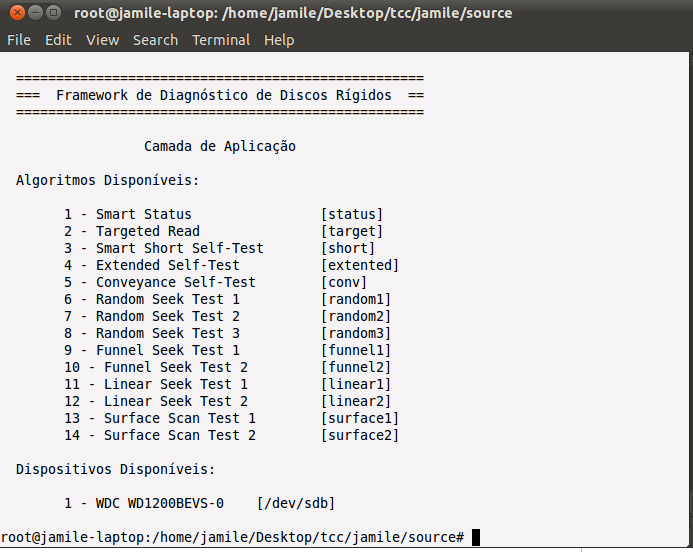
\includegraphics[scale=0.5]{figs/tela.png}
  \caption{Tela inicial da Camada de Aplica��o}
  \label{FIG:telainicial}
\end{figure}

O usu�rio pode obter informa��es sobre os par�metros esperados  executando a op��o \textbf{-h} ou \textbf{--help}.
A tela exibida durante a ajuda � mostrada na Figura \ref{FIG:telahelp}.
\begin{figure}[htb!]
  \centering
  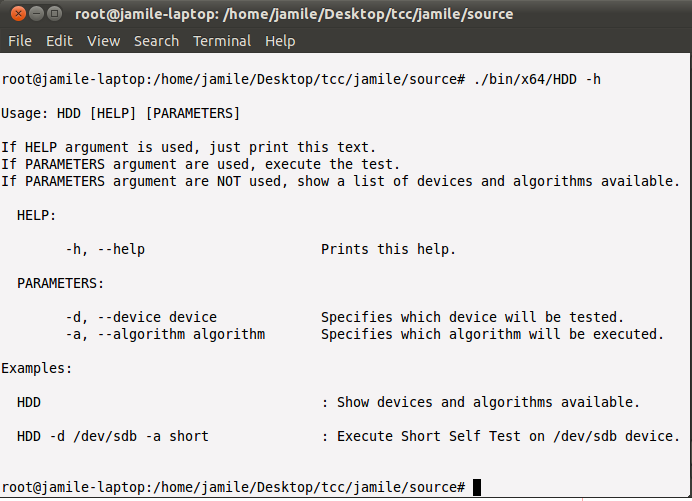
\includegraphics[scale=0.5]{figs/help.png}
  \caption{Tela de ajuda}
  \label{FIG:telahelp}
\end{figure}

A Figura \ref{FIG:telapercent} mostra um algoritmo sendo executado. Para executar um algoritmo, os seguintes par�metros devem ser passados: \textbf{-d} ou \textbf{- -device}  ``disco'' \textbf{-a} ou \textbf{- -algorithm}  ``algoritmo''. No caso da figura os par�metros passados foram: \textbf{ -d /dev/sdb -a short}. O programa ent�o passa a exibir uma barra de progresso com o percentual do teste conclu�do, qual algoritmo est� sendo executado e em que dispositivo.
\begin{figure}[htb!]
  \centering
  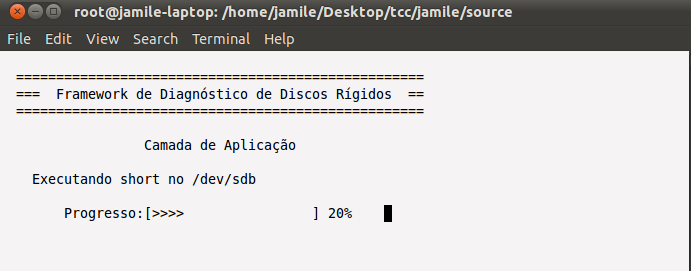
\includegraphics[scale=0.5]{figs/percent.png}
  \caption{Tela de teste em execu��o}
  \label{FIG:telapercent}
\end{figure}

Na conclus�o do teste, o tempo de execu��o � mostrado e o resultado do teste � apresentado, como mostrado na Figura \ref{FIG:telafinal}. O teste mostrado levou 120 segundos e foi conclu�do com sucesso.
\begin{figure}[htb!]
  \centering
  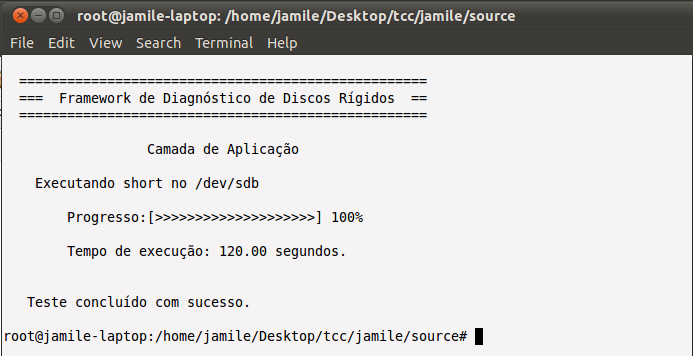
\includegraphics[scale=0.5]{figs/final.png}
  \caption{Tela de teste conclu�do}
  \label{FIG:telafinal}
\end{figure}

\section{Testes}

Nesta se��o s�o apresentados os resultados obtidos com a metodologia descrita no cap�tulo anterior. Para a realiza��o dos testes foram utilizados 12 discos r�gidos, 9 do tipo \ac{HDD} (H1, H2, H3, H4, H5, H6, H7, H8 e H9) e 3 do tipo \ac{SSD} (S1, S2 e S3), com defeitos conhecidos. Cada teste descrito nas tabelas � o resultado obtido na maior parte de 3 execu��es, ou seja, o valor apresentado se repetiu de duas a tr�s vezes.  A nota��o utilizada em todas as tabelas de resultados � descrita na Tabela \ref{TAB:not}. Na Tabela \ref{TAB:ResultsLTTFrame}, os dispositivos testados s�o listados assim como  modelos, \emph{form factors}, capacidades de armazenamento e o resultado obtido testando o dispositivo com outro \emph{software} de diagn�stico.

\begin{table}[htb!]
    \caption{Nota��o utilizada nas tabelas de resultados }
    \label{TAB:not}
    \vspace{-10pt}
    \begin{center}
      \begin{tabular}{|c|c|}
        \hline
        % after \\: \hline or \cline{col1-col2} \cline{col3-col4} ...
        Abrevia��o / S�mbolo & Defini��o \\ \hline
        $\times$ & Teste falhou \\ \hline
        $\checkmark$ & Teste passou \\ \hline
        $\emptyset$ & Teste n�o p�de ser executado \\ \hline
        Short & \ac{SMART} \emph{Short Self-Test} \\ \hline
        Status & \ac{SMART} \emph{Return Status } \\ \hline
        Conv & \ac{SMART} \emph{Conveyance Self-Test} \\ \hline
        Linear1 & \emph{Linear Seek Test 1} \\ \hline
        Linear2 & \emph{Linear Seek Test 2} \\ \hline
        Random1 & \emph{Random Seek Test 1} \\ \hline
        Random2 & \emph{Random Seek Test 2} \\ \hline
        Random3 & \emph{Random Seek Test 3} \\ \hline
        Funnel1 & \emph{Funnel Seek Test 1} \\ \hline
        Funnel2 & \emph{Funnel Seek Test 2} \\ \hline
        Surface1 & \emph{Surface Scan Test 1} \\ \hline
        Surface2 & \emph{Surface Scan Test 2} \\ \hline
        Target & \emph{Targeted Read Test} \\ \hline
      \end{tabular}
    \end{center}
    \vspace{-15pt}
\end{table}

\begin{table}[htb!]
   \caption{Lista dos dispositivos testados}
    \label{TAB:ResultsLTTFrame}
    \vspace{-10pt}
    \begin{center}
       \begin{tabular}{|c|p{5cm}|c|c|c|}
         \hline
         % after \\: \hline or \cline{col1-col2} \cline{col3-col4} ...
         Dispositivo & Modelo & Capacidade & \emph{Form Factor} & PC-Doctor \\ \hline
         H1 &  Seagate ST3500418AS & 500 GB & 3.5'' & $\checkmark$ \\ \hline
         H2 &  Western Digital WD2500AAKX083CA0 & 250GB & 3.5''&$\times$ \\ \hline
         H3 &  Seagate ST31000528AS & 1 TB &  3.5''&$\times$ \\ \hline
         H4 &  Seagate ST3500418AS & 500 GB & 2.5''& $\checkmark$ \\ \hline
         H5 &  Hitachi HTS725050A9A364 & 500 GB  &2.5''& $\times$ \\ \hline
         H6 &  Hitachi HTS545032B9A300 & 320 GB & 2.5''&$\times$ \\ \hline
         H7 & Seagate ST9250315AS & 250 GB  & 2.5''& $\times$ \\ \hline
         H8 & Toshiba MK5061GSY & 500GB &  2.5''&$\times$  \\ \hline
         H9 & Hitachi HTS723232A7A364 & 320 GB  &  2.5''&$\checkmark$   \\ \hline
         S1 & Kingston SNV425S264GB & 64 GB  & 2.5''& $\checkmark$  \\ \hline
         S2 & Toshiba THN5NC128GCSJ & 160 GB &  2.5''&$\times$ \\ \hline
         S3 & Kingston  SV100S264G& 64 GB & 2.5''& $\checkmark$  \\ \hline
       \end{tabular}
    \end{center}
    \vspace{-15pt}
\end{table}

Uma sequ�ncia de execu��o dos algoritmos foi definida com base nos \emph{softwares} do mercado e uma s�rie de hip�teses foi levantada. O primeiro questionamento � relativo � execu��o do \emph{Targeted Read Test}, teste que realiza leituras espec�ficas em regi�es onde algum tipo de problema foi detectado, a fim de determinar qual a melhor ordem de execu��o, no in�cio  ou no final  dos testes.

O segundo questionamento � em rela��o � quantidade de setores checados no algoritmo \emph{Random Seek}. Para responder a este questionamento, o desempenho de tr�s taxas distintas � avaliado.

O terceiro questionamento � quanto � validade da distin��o feita nos algoritmos de \emph{Surface Scan} e \emph{Linear Seek}. Foi avaliado se realizar os testes indo das menores para as maiores LBAs, ou das maiores para as menores LBAs, apresentam varia��es significativas de desempenho.

Por �ltimo, uma hip�tese  � levantada sobre o funcionamento do teste \emph{Funnel Seek}. Saber se, al�m da altern�ncia no sentido de ``crescimento'' da LBA analisada, a leitura de setores mais espec�ficos, como os setores iniciais do disco, que cont�m informa��es sobre a tabela de parti��o\footnote{\ac{MBR}, setor que cont�m a tabela de parti��es do disco e informa��es sobre a inicializa��o do sistema operacional, localizado no setor 0.}, pode influenciar no desempenho do algoritmo.

A ordem de execu��o dos testes definida foi: \emph{Target Read Test}, SMART \emph{Status Test}, SMART \emph{Short Self-Test}, SMART \emph{Conveyance Self-Test}, \emph{Random Seek} 1, 2 e 3, \emph{Funnel Seek} 1 e 2, \emph{Linear Seek} 1 e 2, \emph{Surface Scan} 1 e 2, e \emph{Target Read Test} e os resultados s�o apresentados na Tabela \ref{TAB:ResultsFrame}.

\begin{table}[htb!]
    \caption{Resultados dos Testes.}
    \label{TAB:ResultsFrame}
    \vspace{-10pt}
    \begin{center}
\begin{tabular}{|c|c|c|c|c|c|c|c|c|c|c|c|c|}
  \hline
  % after \\: \hline or \cline{col1-col2} \cline{col3-col4} ...
  Algoritmos & H1 & H2 & H3 & H4 & H5 & H6 & H7 & H8 & H9 & S1 & S2 & S3 \\ \hline
  Status & $\checkmark$ & $\checkmark$ & $\times$ & $\checkmark$ & $\checkmark$ & $\checkmark$ & $\checkmark$ & $\checkmark$ & $\checkmark$ & $\checkmark$  & $\checkmark$ & $\checkmark$ \\ \hline
  Short & $\checkmark$ & $\times$ & $\times$ & $\checkmark$ & $\times$  & $\checkmark$  & $\times$  & $\times$  & $\checkmark$  & $\checkmark$  & $\times$ & $\checkmark$ \\ \hline
  Conv & $\checkmark$  & $\times$ & $\times$ & $\checkmark$ & $\emptyset$ & $\emptyset$ &$\times$ & $\emptyset$ & $\emptyset$ & $\emptyset$ & $\emptyset$ & $\emptyset$ \\ \hline
  Random1 & $\checkmark$  & $\checkmark$  & $\checkmark$  & $\checkmark$  & $\checkmark$  & $\checkmark$  & $\checkmark$  & $\checkmark$  & $\checkmark$  & $\checkmark$  & $\checkmark$ & $\checkmark$ \\ \hline
  Random2 & $\checkmark$  & $\checkmark$  & $\checkmark$  & $\checkmark$  & $\times$  & $\checkmark$  & $\checkmark$  & $\checkmark$  & $\checkmark$  & $\checkmark$  & $\checkmark$ & $\checkmark$ \\ \hline
  Random3 & $\checkmark$  & $\checkmark$  & $\checkmark$  & $\checkmark$  & $\times$  & $\checkmark$  & $\checkmark$  & $\checkmark$  & $\checkmark$  & $\checkmark$  & $\checkmark$ & $\checkmark$ \\ \hline
  Funnel1 & $\checkmark$  & $\checkmark$   & $\checkmark$  & $\checkmark$  & $\checkmark$  & $\checkmark$  & $\times$  & $\checkmark$  & $\checkmark$  & $\checkmark$  & $\checkmark$ & $\checkmark$ \\ \hline
  Funnel2 & $\checkmark$  & $\times$  & $\checkmark$  & $\checkmark$  & $\times$  & $\checkmark$  & $\times$  & $\checkmark$  & $\checkmark$  & $\checkmark$  & $\checkmark$ & $\checkmark$ \\ \hline
  Linear1 & $\checkmark$  & $\checkmark$  & $\checkmark$  & $\checkmark$  & $\checkmark$  & $\checkmark$  & $\checkmark$  & $\checkmark$  & $\checkmark$  & $\checkmark$  & $\checkmark$ & $\checkmark$ \\ \hline
  Linear2 & $\checkmark$  & $\checkmark$  & $\checkmark$  & $\checkmark$  & $\checkmark$  & $\checkmark$  & $\checkmark$  & $\checkmark$  & $\checkmark$  & $\checkmark$  & $\checkmark$ & $\checkmark$ \\ \hline
  Surface1 & $\checkmark$ & $\times$ & $\checkmark$ & $\checkmark$ & $\checkmark$ & $\checkmark$ & $\checkmark$ & $\checkmark$ & $\checkmark$ & $\checkmark$  & $\checkmark$ & $\checkmark$ \\ \hline
  Surface2 & $\checkmark$ & $\times$ & $\checkmark$ & $\checkmark$ & $\checkmark$ & $\checkmark$ & $\checkmark$ & $\times$ & $\checkmark$ & $\checkmark$  & $\checkmark$ & $\checkmark$ \\ \hline
  Target   & $\checkmark$ & $\times$ & $\checkmark$ & $\checkmark$ & $\times$ & $\times$ & $\times$ & $\times$ & $\checkmark$  & $\checkmark$  & $\times$ & $\checkmark$ \\
  \hline
  \end{tabular}
    \end{center}
    \vspace{-15pt}
\end{table}

Os melhores resultados obtidos individualmente foram \emph{SMART Short Self-Test} e \emph{Targeted Read Test}, que detectaram 6 dos 7 dispositivos com falhas. Depois destes est�o o \emph{Funnel Seek 2} e o  \emph{SMART Conveyance Self-Test}, que detectaram sozinhos 3 dos 7 dispositivos falhos. Entretanto, vale salientar que o \emph{SMART Conveyance Self-Test} n�o pode ser executado na maioria dos dispositivos, pois estes n�o t�m suporte a este tipo de teste. Em seguida est� o \emph{Surface Scan 2}, que detectou 2 dos 7 dispositivos falhos e os testes  \emph{Random Seek 2}, \emph{Random Seek 3}, \emph{Funnel Seek 1} e  \emph{Surface Scan 1} que detectaram apenas 1 dos 7 dispositivos falhos. Por �ltimo, est�o  \emph{Random Seek 1}, \emph{Linear Seek 1} e \emph{Linear Seek 2}, que n�o detectaram nenhum dispositivo falho. O alerta de falha dado pelo \emph{SMART Return Status} foi dado apenas para 1 dispositivo e em nenhum dos testes foi observado resultados ``falsos positivos''.

H� importantes pontos a serem analisados. Das tr�s rodadas de testes executadas, a primeira apresentou resultados diferentes entre a execu��o do \emph{Targeted Read Test} no in�cio e no final dos testes. A execu��o inicial detectou apenas 3 dos 7 dispositivos com falhas. Depois da execu��o dos demais testes o \emph{Targeted Read Test} passou a detectar 6 dos 7 dispositivos com falha. Este resultado, da execu��o final, se repetiu nas duas execu��es de cada uma das duas rodadas seguintes. Logo, para o usu�rio � interessante que este teste seja o �ltimo a ser executado.

Este comportamento do \emph{Targeted Read Test} pode ser explicado pela leitura dos \emph{logs} da controladora. Quando outros testes s�o executados, setores com falha podem ser detectados ou, mesmo que o teste n�o seja reprovado, qualquer comportamento estranho que tenha ocorrido ser� registrado no \emph{log} e posteriormente verificado com o \emph{Targeted Read Test}.

 O \emph{Random Seek Test} apresentou baixo desempenho na detec��o de dispositivos com falha, apenas os testes 2 e 3 detectaram 1 dos 7 dispositivos falhos. Entretanto, o desempenho dos algoritmos deve ser analisado conjuntamente e como se trata de um algoritmo fundamentado em aleatoriedade, a realiza��o destes testes com outro conjunto de dispositivos pode apresentar resultados vari�veis.

 Os algoritmos de \emph{Linear Seek} e \emph{Surface Scan} n�o se mostraram eficientes independentemente da ordem de ``crescimento'' das LBAs analisadas, se da menor para a maior ou o contr�rio.

 Um desempenho interessante foi o do \emph{Funnel Seek Test 2}, que se mostrou significativamente melhor que o \emph{Funnel Seek 1}, lembrando que a diferen�a entre eles � a checagem dos 100 primeiros setores do disco feita pelo \emph{Funnel Seek Test 2}.

De maneira geral, o conjunto dos 13 testes implementados foi capaz de detectar os 7 dispositivos defeituosos, alcan�ando assim o resultado obtido utilizando o PC-Doctor.

\section{Tempo de Execu��o}

 Al�m da cobertura de falhas, o tempo de execu��o dos testes deve ser analisado. Na Tabela \ref{TAB:TimeFrame}, s�o apresentados os tempos de execu��o da �ltima rodada dos testes.
\begin{table}[htb!]
    \caption{Tempos de Execu��o dos Testes, em segundos.}                                                                                                         \label{TAB:TimeFrame}
    \vspace{-10pt}
    \begin{center}
\begin{tabular}{|c|c|c|c|c|c|c|c|c|c|c|c|c|}
  \hline
  % after \\: \hline or \cline{col1-col2} \cline{col3-col4} ...
  Algoritmos & H1 & H2 & H3 & H4 & H5 & H6 & H7 & H8 & H9 & S1 & S2 & S3 \\ \hline
  Status & 0 & 1 & 0 & 0 & 0 & 0 & 14 &  0 & 0 & 0  & 1 & 0 \\ \hline
  Short & 81 & 10 & 10 & 60 & 50  & 120  & 24 & 41  &  120  & 50  & 11 & 50 \\ \hline
   Conv & 140  &10 & 10 & 121 & - & - & 24 & -&   - & - & - & - \\ \hline
   Random1 & 106  & 82  & 107  & 106  & 126  & 131  &114  & 83  & 137  & 3  & 1& 1 \\ \hline
   Random2 & 159  & 123  & 162  & 160  & 192  & 196  & 163  &  125 & 205  & 4  & 3 & 2 \\ \hline
   Random3 & 214  & 163  & 250  & 213  & 192  & 262  & 213  &  166  & 274  & 6  & 4 & 4 \\ \hline
   Funnel1 & 129  & 52   & 524  & 129  & 150  & 101  & 18  & 103 & 104  & 0  & 0 & 0 \\ \hline
   Funnel2 & 131  & 52  & 400  & 130  & 150  & 102  & 19  & 104  & 106  & 0  & 1 & 1 \\ \hline
   Linear1 & 49  & 31  & 52  & 47  & 71  & 84 & 67  & 43 &  89  & 3  &2 & 2\\ \hline
   Linear2 & 48  & 32  & 52  & 48  & 72  & 84 & 66  & 44  &  89  & 3  & 2 & 2 \\ \hline
   Surface1 & 535 & 7 & 541 & 533 & 848 & 872 & 677 &  501 & 972 & 36  & 19 & 19 \\ \hline
   Surface2 & 536 & 71 & 543 & 533 & 852 & 873 & 678 &  204 & 968 & 36 & 19 & 19 \\ \hline
   Target   & 1 & 27 & 0 & 0 & 32 & 24 & 10 & 14 &  1  & 0 & 0 & 0 \\                                                                                   \hline                                                                                                                                   \end{tabular}                                                                                                                            \end{center}                                                                                                                       \vspace{-15pt}
\end{table}

Na tabela h� duas grandes ``discrep�ncias'' de tempo: a primeira ocorre entre o tempo levado para executar os testes em dispositivos SSD e a segunda ocorre quando uma falha � encontrada. Neste caso, em uma leitura normal leva-se um tempo maior para o resultado da leitura, pois v�rias tentativas s�o feitas. Entretanto, quando um setor falho � encontrado, a condi��o de parada do algoritmo � satisfeita e ele � encerrado. Como no teste de \emph{Surface Scan 1} do H2, que durou 7 segundos, enquanto que o mesmo teste para o H1, que tem o dobro da capacidade, levou 535 segundos, por exemplo.

 Os testes mais r�pidos foram os de \emph{SMART Return Status} e \emph{Targeted Read}. Em v�rios dispositivos a execu��o levou menos de 1 segundo. Entre os testes de \emph{Random Seek} os testes variaram de 82  a 274 segundos para \acp{HDD} e entre 1 e 6 para \acp{SSD}. Os testes mais demorados foram os de \emph{Surface Scan}, chegando a durar 972 segundos, como no caso do H9. Na Figura \ref{FIG:Tempo_medio}, o tempo m�dio em segundos de cada teste realizado em dispositivos \ac{HDD} (mais demorados) � apresentado.

\begin{figure}[htb]
  \centering
  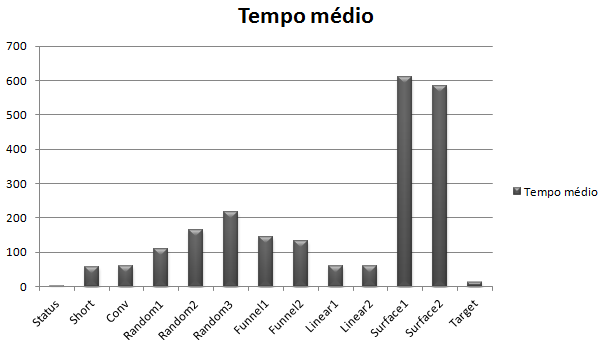
\includegraphics[scale=0.8]{figs/tempo_medio.png}
  \caption{Tempo m�dio dos testes para dispositivos HDD}
  \label{FIG:Tempo_medio}
\end{figure}

Uma sele��o de algoritmos foi feita com base na an�lise dos resultados dos testes e dos tempos de execu��o. Os cinco algoritmos selecionados foram: \emph{SMART Return Status}, \emph{SMART Short Self-Test}, \emph{Random Seek Test 2}, \emph{Funnel Seek Test 2} e \emph{Target Read Test}. Considerando apenas esta combina��o de algoritmos foi poss�vel detectar todos os dispositivos com falha e a soma dos tempos de execu��o foi inferior aos 10 minutos colocados como objetivo para a execu��o de um teste r�pido e eficiente no diagn�stico de discos r�gidos. Na Tabela \ref{TAB:CompFramePCDoc}, os resultados obtidos com esta sele��o de algoritmos e o PC-Doctor foram comparados. Todos os dispositivos defeituosos detectados pelo PC-Doctor tamb�m foram detectados pela sele��o de algoritmos.

\begin{table}[htb!]
    \caption{Compara��o dos Resultados obtidos com a sele��o de algoritmos e o PC-Doctor.}
    \label{TAB:CompFramePCDoc}
    \vspace{-10pt}
    \begin{center}
\begin{tabular}{|c|c|c|c|c|c|c|c|c|c|c|c|c|}
\hline
  % after \\: \hline or \cline{col1-col2} \cline{col3-col4} ...
  Algoritmos & H1 & H2 & H3 & H4 & H5 & H6 & H7 & H8 & H9 & S1 & S2 & S3 \\ \hline
   \hline\hline
  Framework & $\checkmark$ & $\times$ & $\times$ & $\checkmark$ & $\times$ & $\times$ & $\times$ & $\times$ & $\checkmark$  & $\checkmark$  & $\times$ & $\checkmark$ \\
  \hline\hline
  PC-Doctor & $\checkmark$ & $\times$ & $\times$ & $\checkmark$ & $\times$ & $\times$ & $\times$ & $\times$ & $\checkmark$  & $\checkmark$  & $\times$ & $\checkmark$ \\
  \hline \hline
  \end{tabular}
    \end{center}
    \vspace{-15pt}
\end{table}

O \emph{SMART Return Status} foi escolhido por ser um importante sinalizador  da ``sa�de'' do dispositivo. O \emph{SMART Short Self-Test} e o \emph{Target Read Test} foram escolhidos por terem apresentado a melhor capacidade de detec��o de falhas  entre os algoritmos avaliados. Por fim,  o \emph{Random Seek Test 2} e o \emph{Funnel Seek Test 2} foram escolhidos por terem apresentado uma capacidade mediana de detec��o e  servirem de complemento ao \emph{Target Read Test}.

\section{Resumo do Cap�tulo}

Neste cap�tulo foram apresentados os resultados obtidos no desenvolvimento do \emph{Framework} proposto: a cria��o de um programa capaz de executar testes de diagn�stico e que possibilitou a an�lise de algoritmos de teste  e a sele��o dos algoritmos mais eficientes com base na an�lise realizada.

No pr�ximo cap�tulo s�o apresentadas as conclus�es e propostas de continua��o deste trabalho. 
%%%%%%%%%%%%%%%%%%%%iron %%%%%%%%%%%%%%%%%%%%%%%%%%%%%%%%%%%%%%%%%%%%%
%%%% CAP�TULO 8: Conclus�es
\chapter{Conclus�o}

Neste trabalho foi desenvolvido um \emph{framework} para dar suporte ao desenvolvimento de testes de diagn�stico de discos r�gidos usados em computadores pessoais. Utilizou-se o sistema Linux pois, mesmo sendo empregado  por uma pequena parcela do mercado, possibilita a realiza��o de testes em computadores com qualquer sistema operacional instalado, bastando apenas a reinicializa��o.

O programa desenvolvido com a camada de aplica��o, criada utilizando o \emph{framework} apresentado neste trabalho, mostrou-se bastante eficiente pois apresentou desempenho similar aos das ferramentas de diagn�stico do mercado. Todos os dispositivos com falhas foram detectados, utilizando apenas uma combina��o de 5 testes, com tempo de execu��o inferior a 10 minutos.

Entretanto, a maior contribui��o deste trabalho est� n�o apenas na an�lise realizada da efici�ncia dos algoritmos de testes, mas em  fornecer os recursos necess�rios para  a implementa��o de novos algoritmos de maneira simples, como os principais comandos necess�rios, uma camada de aplica��o que encapsula estes comandos e um m�todo de inser��o de falhas, �til na valida��o de novos comandos e algoritmos de teste.

Durante o desenvolvimento deste trabalho, algumas dificuldades foram enfrentadas, principalmente devido � documenta��o dos padr�es \ac{ATA} e \ac{SCSI}, que se mostrou superficial e mal organizada. H� livros que se dedicam a fazer uma an�lise mais detalhada destes padr�es, entretanto os mesmos s�o antigos e est�o um pouco defasados. Para contornar este empecilho, v�rios testes e experimentos foram realizados para tentar deduzir, atrav�s de investiga��o, o comportamento que n�o era descrito pela documenta��o.

\section{Perspectivas Futuras}


Este trabalho pode ser continuado de diversas maneiras. Pode-se trabalhar na implementa��o de mais comandos \ac{SCSI}, visando dar cobertura tamb�m a discos \ac{SAS} e a servidores. A interface gr�fica deve ser aprimorada, para que se torne mais robusta e mais  agrad�vel de ser utilizada. Por fim, a principal vertente de continua��o deste trabalho � o  desenvolvimento de novos algoritmos e o aprimoramento dos testes implementados aqui, com a realiza��o de mais rodadas de teste e a experimenta��o de novos par�metros em um conjunto maior de discos r�gidos.


%%%%%%%%%%%%%%%%%%%%%%%%%%%%%%%%%%%%%%%%%%%%%%%%%%%%%%%%%%%%%%%%%
%%% AP\^{E}NDICE
%\appendix
%\begin{appendices}
%\chapter{Exemplo Comando Inquiry} \label{APX:ATA}

MATS:

\begin{table}[!ht]
\caption{\emph{MATS.}}
\centering
\label{TAB:MATS}
\begin{tabular}{| c | l r |}
\hline
1 & W0 & $\Updownarrow$ \\
2 & R0, W1 & $\Updownarrow$ \\
3 & R1 & $\Updownarrow$ \\
\hline
\end{tabular}
\end{table}


%%\chapter{Cria��o de Bootable} \label{APX:SCSI}

\begin{verbatim}
Customize Live Environment

This procedure is almost identical to customizing a LiveCD (up to the generation of the .squashfs image). Please see LiveCDCustomization for detailed instructions on customizing the LiveCD. I will only be providing a basic rundown on the process.

Extract /casper/filesystem.squashfs to /casper/chroot/

sudo mount -o loop -t squashfs /casper/filesystem.squashfs /mnt
sudo mkdir /casper/chroot
sudo rsync -ax /mnt/. /casper/chroot/.
sudo umount /mnt
Regenerate initrd.gz
Since we edited bootup scripts, we need to regenerate the file we know as /casper/initrd.gz to incorporate these changes:


sudo cp -L /etc/resolv.conf /casper/chroot/etc/
sudo mount -t proc none /casper/chroot/proc
sudo mount -o bind /dev /casper/chroot/dev
sudo chroot /casper/chroot /bin/bash
At this point, you are "in" the live environment's filesystem. We will be doing this a few more times before the day is over. Remember that our Live environment is at /casper/chroot, not at edit/ (adjust customization commands accordingly).

Optional: Customize Live Environment Further

It would be a great idea to add or remove some packages, or add some default user settings, etc, to make the live environment friendlier. The previously linked LiveCD customization article provides full details on how to do a wide variety of customizations. Follow those instructions, up to: "Putting the CD together" (don't do that step). Instead, replace it with

Ideas for customizations specific to this howto include:

Removing behemoth packages like OpenOffice.

Adding proprietary 3D video drivers by default (TODO: expand on this idea)
Removing shutdown scripts (TODO: expand)
Customizing user default settings in /etc/skel, including importing a firefox profile, etc. The LiveCD howto roughly states how to do this. (TODO: expand)
Suppress the eject notice at shutdown.

rm /etc/rc?.d/*casper*
Install something like sshfs so you can easily use SSH-able systems as permanent storage (TODO: Expand)
Upgrade the whole system and regenerate initrd.gz


apt-get update
apt-get dist-upgrade
apt-get autoclean
apt-get autoremove
apt-get clean
mkinitramfs -o /new-initrd.gz 2.6.31-16-generic
exit
umount -l /casper/chroot/dev
umount -l /casper/chroot/proc
The mkinitramfs command may take 30 seconds to a few minutes, depending on your CPU speed. The exit command will take you back to your original shell, that's not within with live environment. Now we will move this initrd to the right spot:


sudo mv /casper/chroot/new-initrd.gz /casper/initrd.gz
sudo mksquashfs /casper/chroot /casper/filesystem.squashfs -noappend -always-use-fragments
The always-use-fragments argument allows space to be used more efficiently, at the cost of more seeking. Since our image is to be loaded into RAM, seeking is costless and not a concern as opposed to on a mechanical medium.


title Jaunty RAM Session
kernel /casper/vmlinuz boot=casper toram splash
initrd /casper/initrd.gz
Reboot and Enjoy


\end{verbatim}
%
%\begin{verbatim}
%    D - Direct Access Block Device (SBC-3)            Device Column key
%    .T - Sequential Access Device (SSC-3)             ---------------------
%    . L - Printer Device (SSC)                        M = Mandatory
%    .  P - Processor Device (SPC-2)                   O = Optional
%    .  .W - Write Once Block Device (SBC)             V = Vendor specific
%    .  . R - C/DVD Device (MMC-6)                     Z = Obsolete -- with
%    .  .  O - Optical Memory Block Device (SBC)           [std] identifying
%    .  .  .M - Media Changer Device (SMC-3)               last standard
%    .  .  . A - Storage Array Device (SCC-2)
%    .  .  .  E - SCSI Enclosure Services device (SES-2)
%    .  .  .  .B - Simplified Direct-Access (Reduced Block) device (RBC)
%    .  .  .  . K - Optical Card Reader/Writer device (OCRW)
%    .  .  .  .  V - Automation/Device Interface device (ADC-2)
%    .  .  .  .  .F - Object-based Storage Device (OSD-2)
%    .  .  .  .  .
%OP  DTLPWROMAEBKVF  Description
%00  MMMMMMMMMMMMMM  TEST UNIT READY
%01   M              REWIND
%01  Z V ZZZZ        REZERO UNIT [SBC]
%02  VVVVVV V
%03  MMMMMMMMMMOMMM  REQUEST SENSE
%04  M    OO         FORMAT UNIT
%%04   O              FORMAT MEDIUM
%%OP  DTLPWROMAEBKVF  Description
%%04    O             FORMAT
%%05  VMVVVV V        READ BLOCK LIMITS
%%06  VVVVVV V
%%07  OVV O OV        REASSIGN BLOCKS
%%07         O        INITIALIZE ELEMENT STATUS
%%08  MMV O OV        READ(6)
%%08     O            RECEIVE
%%08                  GET MESSAGE(6)
%%09  VVVVVV V
%%0A  OO  O OV        WRITE(6)
%%0A     M            SEND(6)
%%0A                  SEND MESSAGE(6)
%%0A    M             PRINT
%%0B  Z   ZOZV        SEEK(6) [SBC]
%%0B   O              SET CAPACITY
%%0B    O             SLEW AND PRINT
%%0C  VVVVVV V
%%0D  VVVVVV V
%%0E  VVVVVV V
%%0F  VOVVVV V        READ REVERSE(6)
%%10  VM VVV          WRITE FILEMARKS(6)
%%10    O             SYNCHRONIZE BUFFER
%%11  VMVVVV          SPACE(6)
%%12  MMMMMMMMMMMMMM  INQUIRY
%%13  V VVVV
%%13   O              VERIFY(6)
%%14  VOOVVV          RECOVER BUFFERED DATA
%%15  OMO O OOOO OO   MODE SELECT(6)
%%16  ZZMZO OOOZ O    RESERVE(6) [SPC-2]
%%16         Z        RESERVE ELEMENT(6) [SMC]
%%17  ZZMZO OOOZ O    RELEASE(6) [SPC-2]
%%17         Z        RELEASE ELEMENT(6) [SMC]
%%18  ZZZZOZO    Z    COPY [SPC]
%%19  VMVVVV          ERASE(6)
%%OP  DTLPWROMAEBKVF  Description
%%1A  OMO O OOOO OO   MODE SENSE(6)
%%1B  O   OOO O MO O  START STOP UNIT
%%1B   O          M   LOAD UNLOAD
%%1B                  SCAN
%%1B    O             STOP PRINT
%%1B         O        OPEN/CLOSE IMPORT/EXPORT ELEMENT
%%1C  OOOOO OOOM OOO  RECEIVE DIAGNOSTIC RESULTS
%%1D  MMMMM MMOM MMM  SEND DIAGNOSTIC
%%1E  OO  OOOO   O O  PREVENT ALLOW MEDIUM REMOVAL
%%1F
%%20  V   VVV    V
%%21  V   VVV    V
%%22  V   VVV    V
%%23  V   V V    V
%%23       O          READ FORMAT CAPACITIES
%%24  V   VV          SET WINDOW
%%25  M   M M   M     READ CAPACITY(10)
%%25       O          READ CAPACITY
%%25             M    READ CARD CAPACITY
%%25                  GET WINDOW
%%26  V   VV
%%27  V   VV
%%28  M   MOM   MM    READ(10)
%%28                  GET MESSAGE(10)
%%29  V   VVO         READ GENERATION
%%2A  O   MOM   MO    WRITE(10)
%%2A                  SEND(10)
%%2A                  SEND MESSAGE(10)
%%2B  Z   OOO    O    SEEK(10) [SBC]
%%2B   M              LOCATE(10)
%%2B         O        POSITION TO ELEMENT
%%2C  V    OO         ERASE(10)
%%2D        O         READ UPDATED BLOCK
%%2D  V
%%OP  DTLPWROMAEBKVF  Description
%%2E  O   OOO   MO    WRITE AND VERIFY(10)
%%2F  O   OOO         VERIFY(10)
%%30  Z   ZZZ         SEARCH DATA HIGH(10) [SBC]
%%31  Z   ZZZ         SEARCH DATA EQUAL(10) [SBC]
%%31                  OBJECT POSITION
%%32  Z   ZZZ         SEARCH DATA LOW(10) [SBC]
%%33  Z   OZO         SET LIMITS(10) [SBC]
%%34  O   O O    O    PRE-FETCH(10)
%%34   M              READ POSITION
%%34                  GET DATA BUFFER STATUS
%%35  O   OOO   MO    SYNCHRONIZE CACHE(10)
%%36  Z   O O    O    LOCK UNLOCK CACHE(10) [SBC]
%%37  O     O         READ DEFECT DATA(10)
%%37         O        INITIALIZE ELEMENT STATUS WITH RANGE
%%38      O O    O    MEDIUM SCAN
%%39  ZZZZOZO    Z    COMPARE [SPC]
%%3A  ZZZZOZO    Z    COPY AND VERIFY [SPC]
%%3B  OOOOOOOOOOMOOO  WRITE BUFFER
%%3C  OOOOOOOOOO OOO  READ BUFFER
%%3D        O         UPDATE BLOCK
%%3E  O   O O         READ LONG(10)
%%3F  O   O O         WRITE LONG(10)
%%OP  DTLPWROMAEBKVF  Description
%%40  ZZZZOZOZ        CHANGE DEFINITION [SPC]
%%41  O               WRITE SAME(10)
%%42  O               UNMAP
%%42       O          READ SUB-CHANNEL
%%43       O          READ TOC/PMA/ATIP
%%44   M          M   REPORT DENSITY SUPPORT
%%44                  READ HEADER
%%45       O          PLAY AUDIO(10)
%%46       M          GET CONFIGURATION
%%47       O          PLAY AUDIO MSF
%%48  O         O     SANITIZE
%%OP  DTLPWROMAEBKVF  Description
%%49
%%4A       M          GET EVENT STATUS NOTIFICATION
%%4B       O          PAUSE/RESUME
%%4C  OOOOO OOOO OOO  LOG SELECT
%%4D  OOOOO OOOO OMO  LOG SENSE
%%4E       O          STOP PLAY/SCAN
%%4F
%%50  O               XDWRITE(10)
%%51  O               XPWRITE(10)
%%51       O          READ DISC INFORMATION
%%52  O               XDREAD(10)
%%52       O          READ TRACK INFORMATION
%%53  O               XDWRITEREAD(10)
%%53       O          RESERVE TRACK
%%54       O          SEND OPC INFORMATION
%%55  OOO OMOOOOMOMO  MODE SELECT(10)
%%56  ZZMZO OOOZ      RESERVE(10) [SPC-2]
%%56         Z        RESERVE ELEMENT(10) [SMC]
%%57  ZZMZO OOOZ      RELEASE(10) [SPC-2]
%%57         Z        RELEASE ELEMENT(10) [SMC]
%%58       O          REPAIR TRACK
%%59
%%5A  OOO OMOOOOMOMO  MODE SENSE(10)
%%5B       O          CLOSE TRACK/SESSION
%%5C       O          READ BUFFER CAPACITY
%%5D       O          SEND CUE SHEET
%%5E  OMOOO OOOO   M  PERSISTENT RESERVE IN
%%5F  OMOOO OOOO   M  PERSISTENT RESERVE OUT
%%7E  OO   O OOOO O   extended CDB
%%7F  O            M  variable length CDB (more than 16 bytes)
%%80  Z               XDWRITE EXTENDED(16) [SBC]
%%80   M              WRITE FILEMARKS(16)
%%81  Z               REBUILD(16) [SBC]
%%81   O              READ REVERSE(16)
%%OP  DTLPWROMAEBKVF  Description
%%82  Z               REGENERATE(16) [SBC]
%%82   O              ALLOW OVERWRITE
%%83  OOOOO O    OO   EXTENDED COPY
%%84  OOOOO O    OO   RECEIVE COPY RESULTS
%%85  O    O    O     ATA PASS THROUGH(16)
%%86  OO OO OOOOOOO   ACCESS CONTROL IN
%%87  OO OO OOOOOOO   ACCESS CONTROL OUT
%%88  MO  O O   O     READ(16)
%%89  O               COMPARE AND WRITE
%%8A  OO  O O   O     WRITE(16)
%%8B  O               ORWRITE
%%8C  OO  O OO  O M   READ ATTRIBUTE
%%8D  OO  O OO  O O   WRITE ATTRIBUTE
%%8E  O   O O   O     WRITE AND VERIFY(16)
%%8F  OO  O O   O     VERIFY(16)
%%90  O   O O   O     PRE-FETCH(16)
%%91  O   O O   O     SYNCHRONIZE CACHE(16)
%%91   O              SPACE(16)
%%92  Z   O O         LOCK UNLOCK CACHE(16) [SBC]
%%92   M              LOCATE(16)
%%93  O               WRITE SAME(16)
%%93   M              ERASE(16)
%%94 [usage proposed by SCSI Socket Services project]
%%95 [usage proposed by SCSI Socket Services project]
%%96 [usage proposed by SCSI Socket Services project]
%%97 [usage proposed by SCSI Socket Services project]
%%98
%%99
%%9A
%%9B
%%9C
%%9D
%%9E                  SERVICE ACTION IN(16)
%%9F              M   SERVICE ACTION OUT(16)
%%OP  DTLPWROMAEBKVF  Description
%%A0  MMOOO OMMM OMO  REPORT LUNS
%%A1       O          BLANK
%%A1  O         O     ATA PASS THROUGH(12)
%%A2  OO   O      O   SECURITY PROTOCOL IN
%%A3  OOO O OOMOOOM   MAINTENANCE (IN)
%%A3       O          SEND KEY
%%A4  OOO O OOOOOOO   MAINTENANCE (OUT)
%%A4       O          REPORT KEY
%%A5   Z  O OM        MOVE MEDIUM [SMC-2]
%%A5       O          PLAY AUDIO(12)
%%A6         O        EXCHANGE MEDIUM
%%A6       O          LOAD/UNLOAD C/DVD
%%A7  ZZ  O O         MOVE MEDIUM ATTACHED [SMC-2]
%%A7       O          SET READ AHEAD
%%A8  O   OOO         READ(12)
%%A8                  GET MESSAGE(12)
%%A9              O   SERVICE ACTION OUT(12)
%%AA  O   OOO         WRITE(12)
%%AA                  SEND MESSAGE(12)
%%AB       O      O   SERVICE ACTION IN(12)
%%AC        O         ERASE(12)
%%AC       O          GET PERFORMANCE
%%AD       O          READ DVD STRUCTURE
%%AE  O   O O         WRITE AND VERIFY(12)
%%AF  O   O O         VERIFY(12)
%%B0      ZZZ         SEARCH DATA HIGH(12) [SBC]
%%B1      ZZZ         SEARCH DATA EQUAL(12) [SBC]
%%B2      ZZZ         SEARCH DATA LOW(12) [SBC]
%%B3  Z   OZO         SET LIMITS(12) [SBC]
%%B4  ZZ  OZO         READ ELEMENT STATUS ATTACHED [SMC-2]
%%B5  OO   O      O   SECURITY PROTOCOL OUT
%%B5         O        REQUEST VOLUME ELEMENT ADDRESS
%%B6         O        SEND VOLUME TAG
%%B6       O          SET STREAMING
%%OP  DTLPWROMAEBKVF  Description
%%B7  O     O         READ DEFECT DATA(12)
%%B8   Z  OZOM        READ ELEMENT STATUS [SMC-2]
%%B9       O          READ CD MSF
%%BA  O   O OOMO      REDUNDANCY GROUP (IN)
%%BA       O          SCAN=�-
%%BB  O   O OOOO      REDUNDANCY GROUP (OUT)
%%BB       O          SET CD SPEED
%%BC  O   O OOMO      SPARE (IN)
%%BD  O   O OOOO      SPARE (OUT)
%%BD       O          MECHANISM STATUS
%%BE  O   O OOMO      VOLUME SET (IN)
%%BE       O          READ CD
%%BF  O   O OOOO      VOLUME SET (OUT)
%%BF       O          SEND DVD STRUCTURE
%\end{verbatim} 
%\end{appendices}
%%%%%%%%%%%%%%%%%%%%%%%%%%%%%%%%%%%%%%%%%%%%%%%%%%%%%%%%%%%%%%%%%
%%%% INDICE REMISSIVO
%%%%%%%%%%%%%%%%%%%%%%%%%%%%%%%%%%%%%%%%%%%%%%%%%%%%%%%%%%%%%%%%%
%%%% GLOSS\'{A}RIO
%%%%%%%%%%%%%%%%%%%%%%%%%%%%%%%%%%%%%%%%%%%%%%%%%%%%%%%%%%%%%%%%%
%%%% REFER\^{E}NCIAS BIBLIOGR\'{A}FICAS
%\bibliographystyle{abnt-alf}
%\usepackage[num]{abntcite}
%\bibliographystyle{abnt-alf}
%\bibliographystyle{plain}

\addcontentsline{toc}{chapter}{\bibname}
%\bibliography{referencias}
\end{document}
